% Chapter Template

\chapter{Ensayos y resultados} % Main chapter title

\label{Chapter4} % Change X to a consecutive number; for referencing this chapter elsewhere, use \ref{ChapterX}

En este capítulo se presentan los ensayos realizados al trabajo y los resultados obtenidos. Inicialmente, se introducen los ensayos realizados sobre el hardware con un mínimo de bloques de software. Luego, se detallan diferentes ensayos de integración a través del uso de técnicas de \textit{testing} de máquinas de estados finitos.

%----------------------------------------------------------------------------------------
%	SECTION 1
%----------------------------------------------------------------------------------------

\section{Pruebas funcionales de hardware}
\label{sec:pruebasHW}

Las pruebas de hardware se dividieron en tres etapas:

\begin{enumerate}
\item Ensayos sobre \textit{protoboard}. 
\item Primer ensayo de integración, donde los módulos fueron montados sobre una base de madera. 
\item Ensayo final de integración con los elementos montados en los gabinetes.
\end{enumerate}

En la figura \ref{fig:Protoboard} se muestra el banco de pruebas para el sensor de tensión, el \textit{display} y el módulo RS-232 utilizados en los ensayos sobre \textit{protoboard}.

\begin{figure}[htpb]
	\centering
	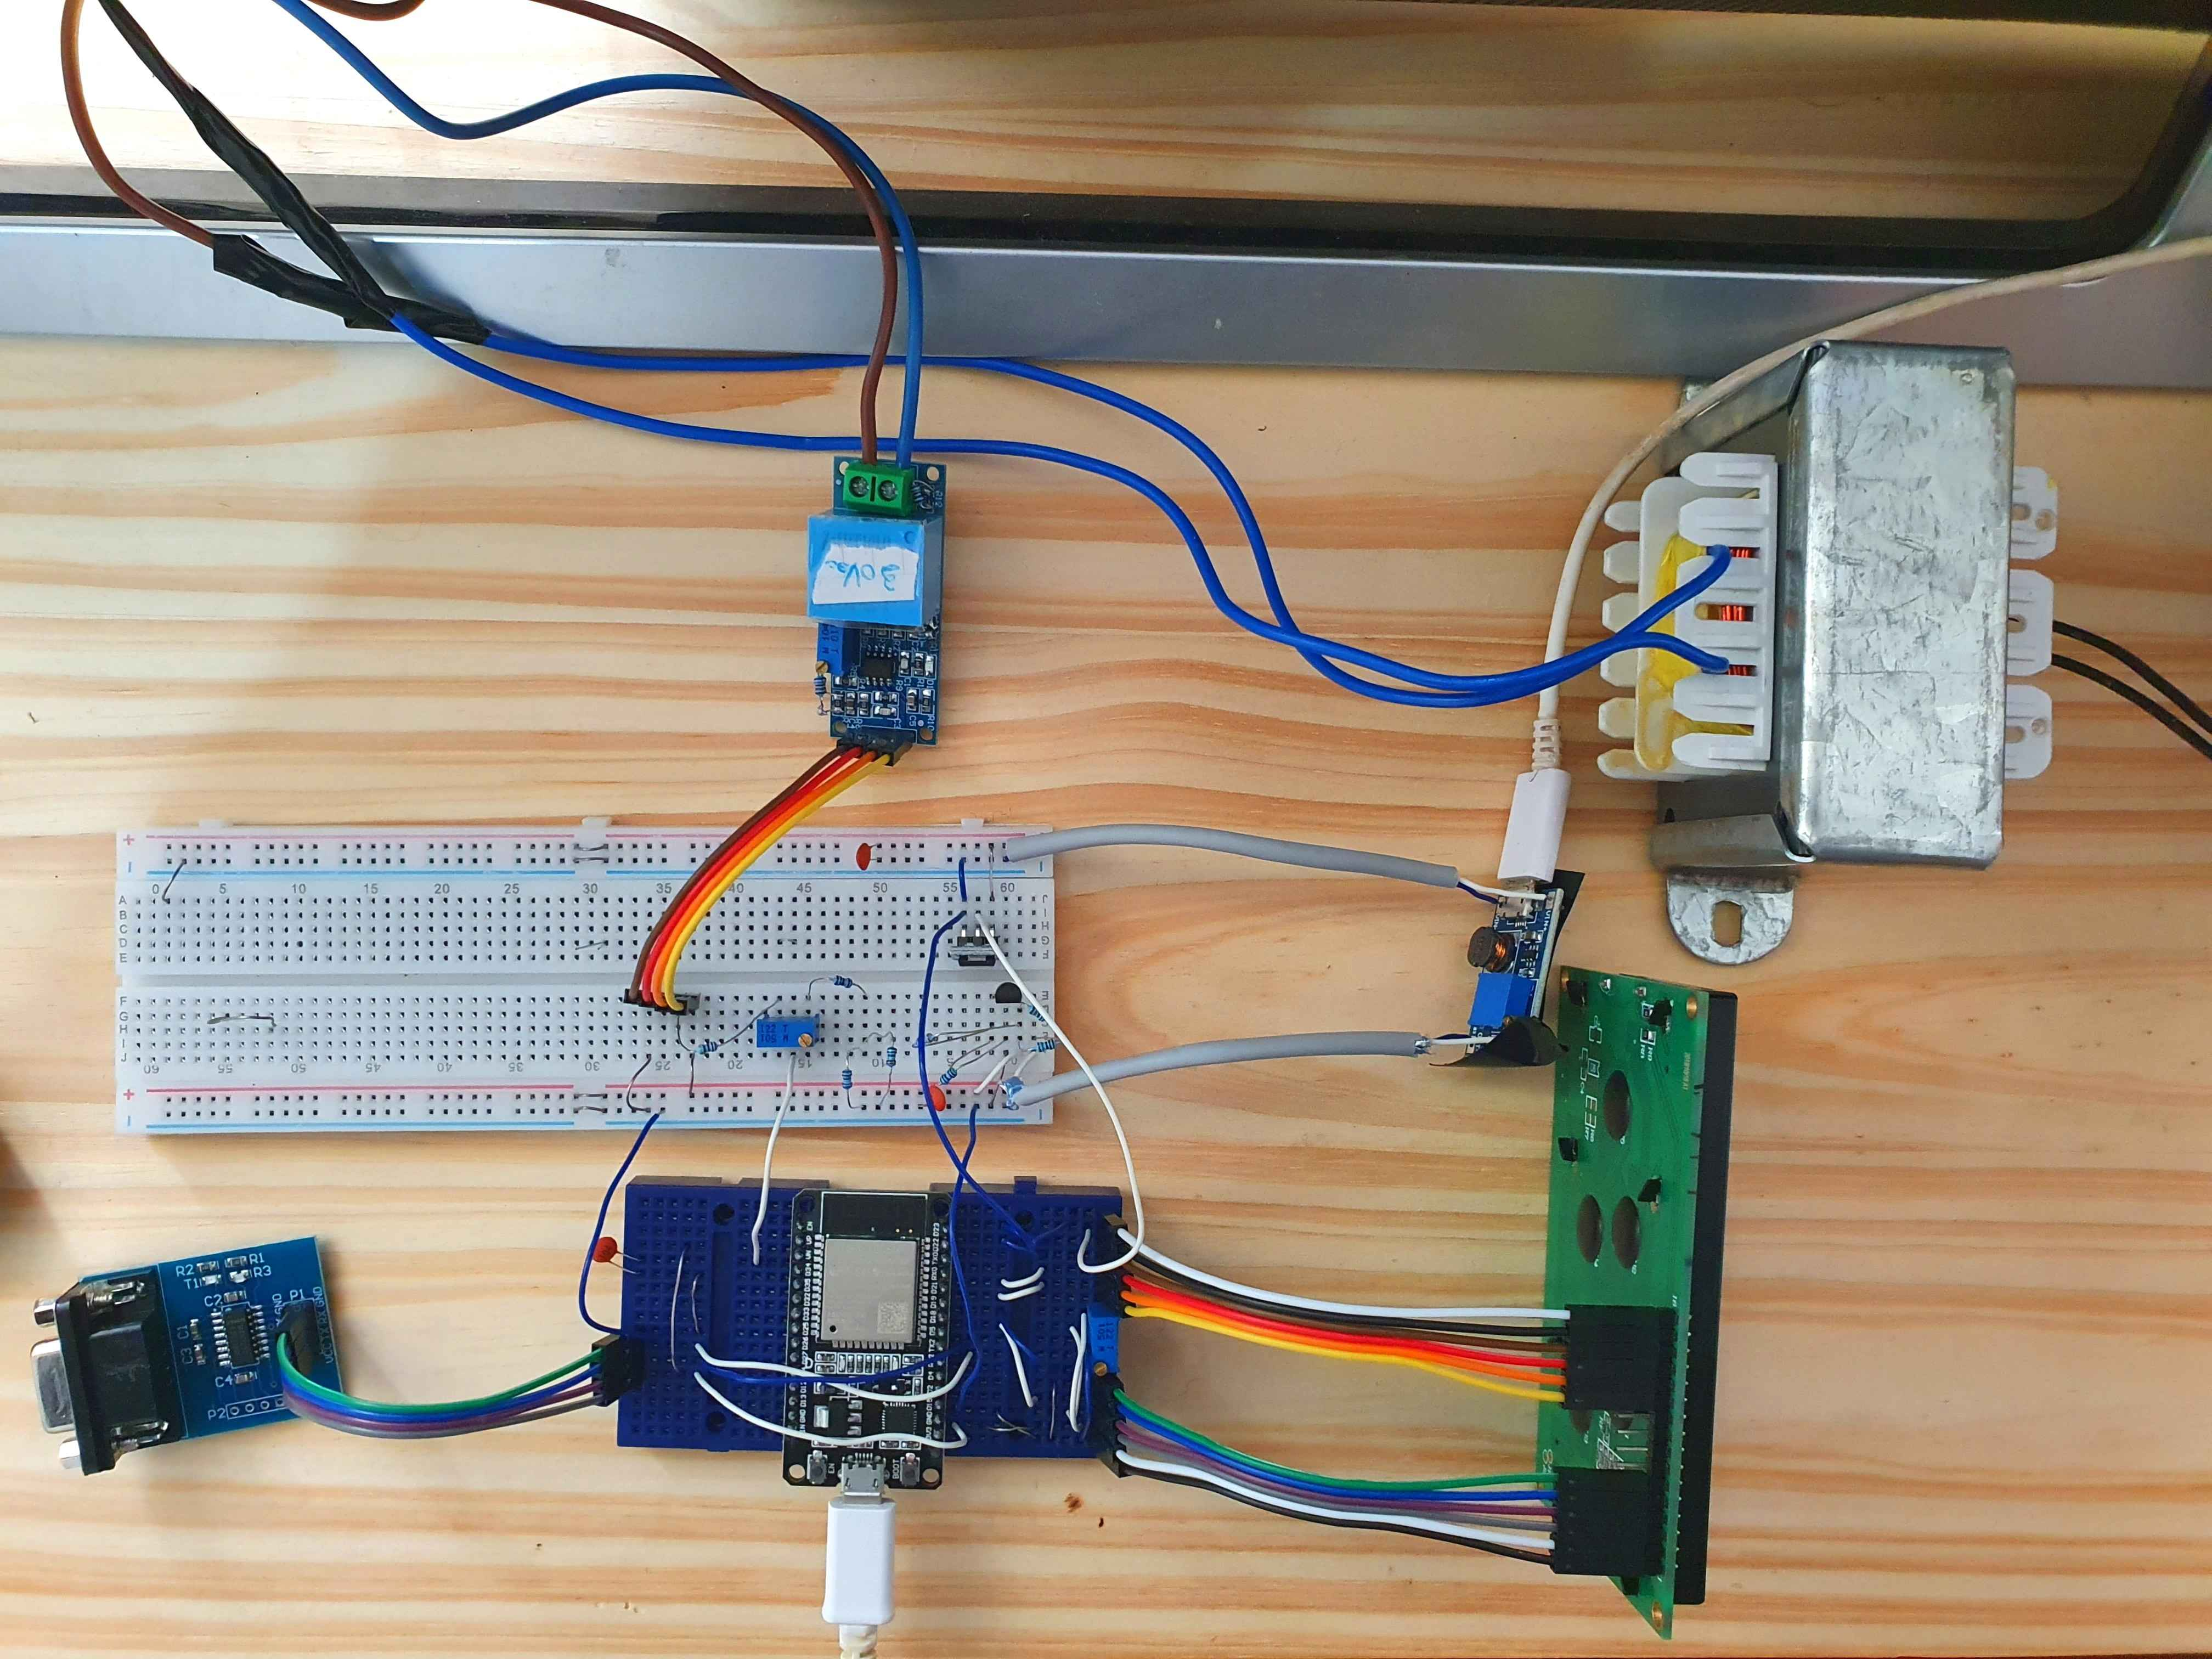
\includegraphics[scale=0.09]{./Figures/protoboard.jpg}
	\caption{Ensayos sobre \textit{protoboard}.}
	\label{fig:Protoboard}
\end{figure}

En los ensayos sobre \textit{protoboard}, se realizaron pruebas sobre los módulos individuales con bloques de firmware reducidos. Las pruebas principales se detallan a continuación:
\begin{enumerate}
	\item Pruebas de los módulos sensores de tensión y corriente.
	\item Pruebas del \textit{display}.
	\item Pruebas sobre la interfaz RS-232 utilizando un terminal.
\end{enumerate}

Para las pruebas sobre los módulos sensores de tensión y corriente se utilizaron los siguientes instrumentos:
\begin{itemize}
\item Multímetro. Marca: Pro'sKit, modelo: MT-1232 \citep{MT1232}.
\item Osciloscopio. Marca: OWON, modelo: VDS3102  \citep{VDS3102}.
\end{itemize}

A partir de estos instrumentos, se realizaron mediciones para constatar la exactitud y repetitividad de los módulos sensores, así como, para ajustar los potenciometros y entregar tensiones acorde para las entradas del ADC del microcontrolador. A modo de ejemplo, en la figura \ref{fig:ISOsc}, se muestra una captura de pantalla de la tensión entregada por el módulo sensor de corriente para el bobinado secundario.

\begin{figure}[htpb]
	\centering
	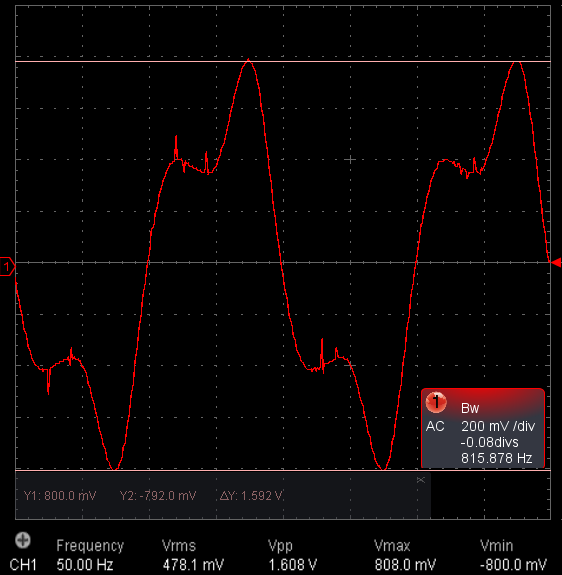
\includegraphics[scale=0.6]{./Figures/osc_is.png}
	\caption{Medición de corriente en el bobinado secundario.}
	\label{fig:ISOsc}
\end{figure}

Luego de validar los módulos de hardware individualmente sobre el \textit{protoboard}, se procedió a montarlos sobre una base de madera y a construir la placa universal. Esta nueva etapa permitió comenzar a trabajar en las pruebas de integración sin necesidad de contar con los gabinetes totalmente ensamblados. Se decidió realizar esta etapa intermedia porque los ensayos en \textit{protoboard} no eran aptos para la gran cantidad de módulos a conectar y, además, representaba un riesgo grande ya que varios módulos están conectados a 220 V$_{RMS}$. En la figura \ref{fig:BaseMadera}, se observa la base de madera con varios módulos montados sobre ella.

\begin{figure}[htpb]
	\centering
	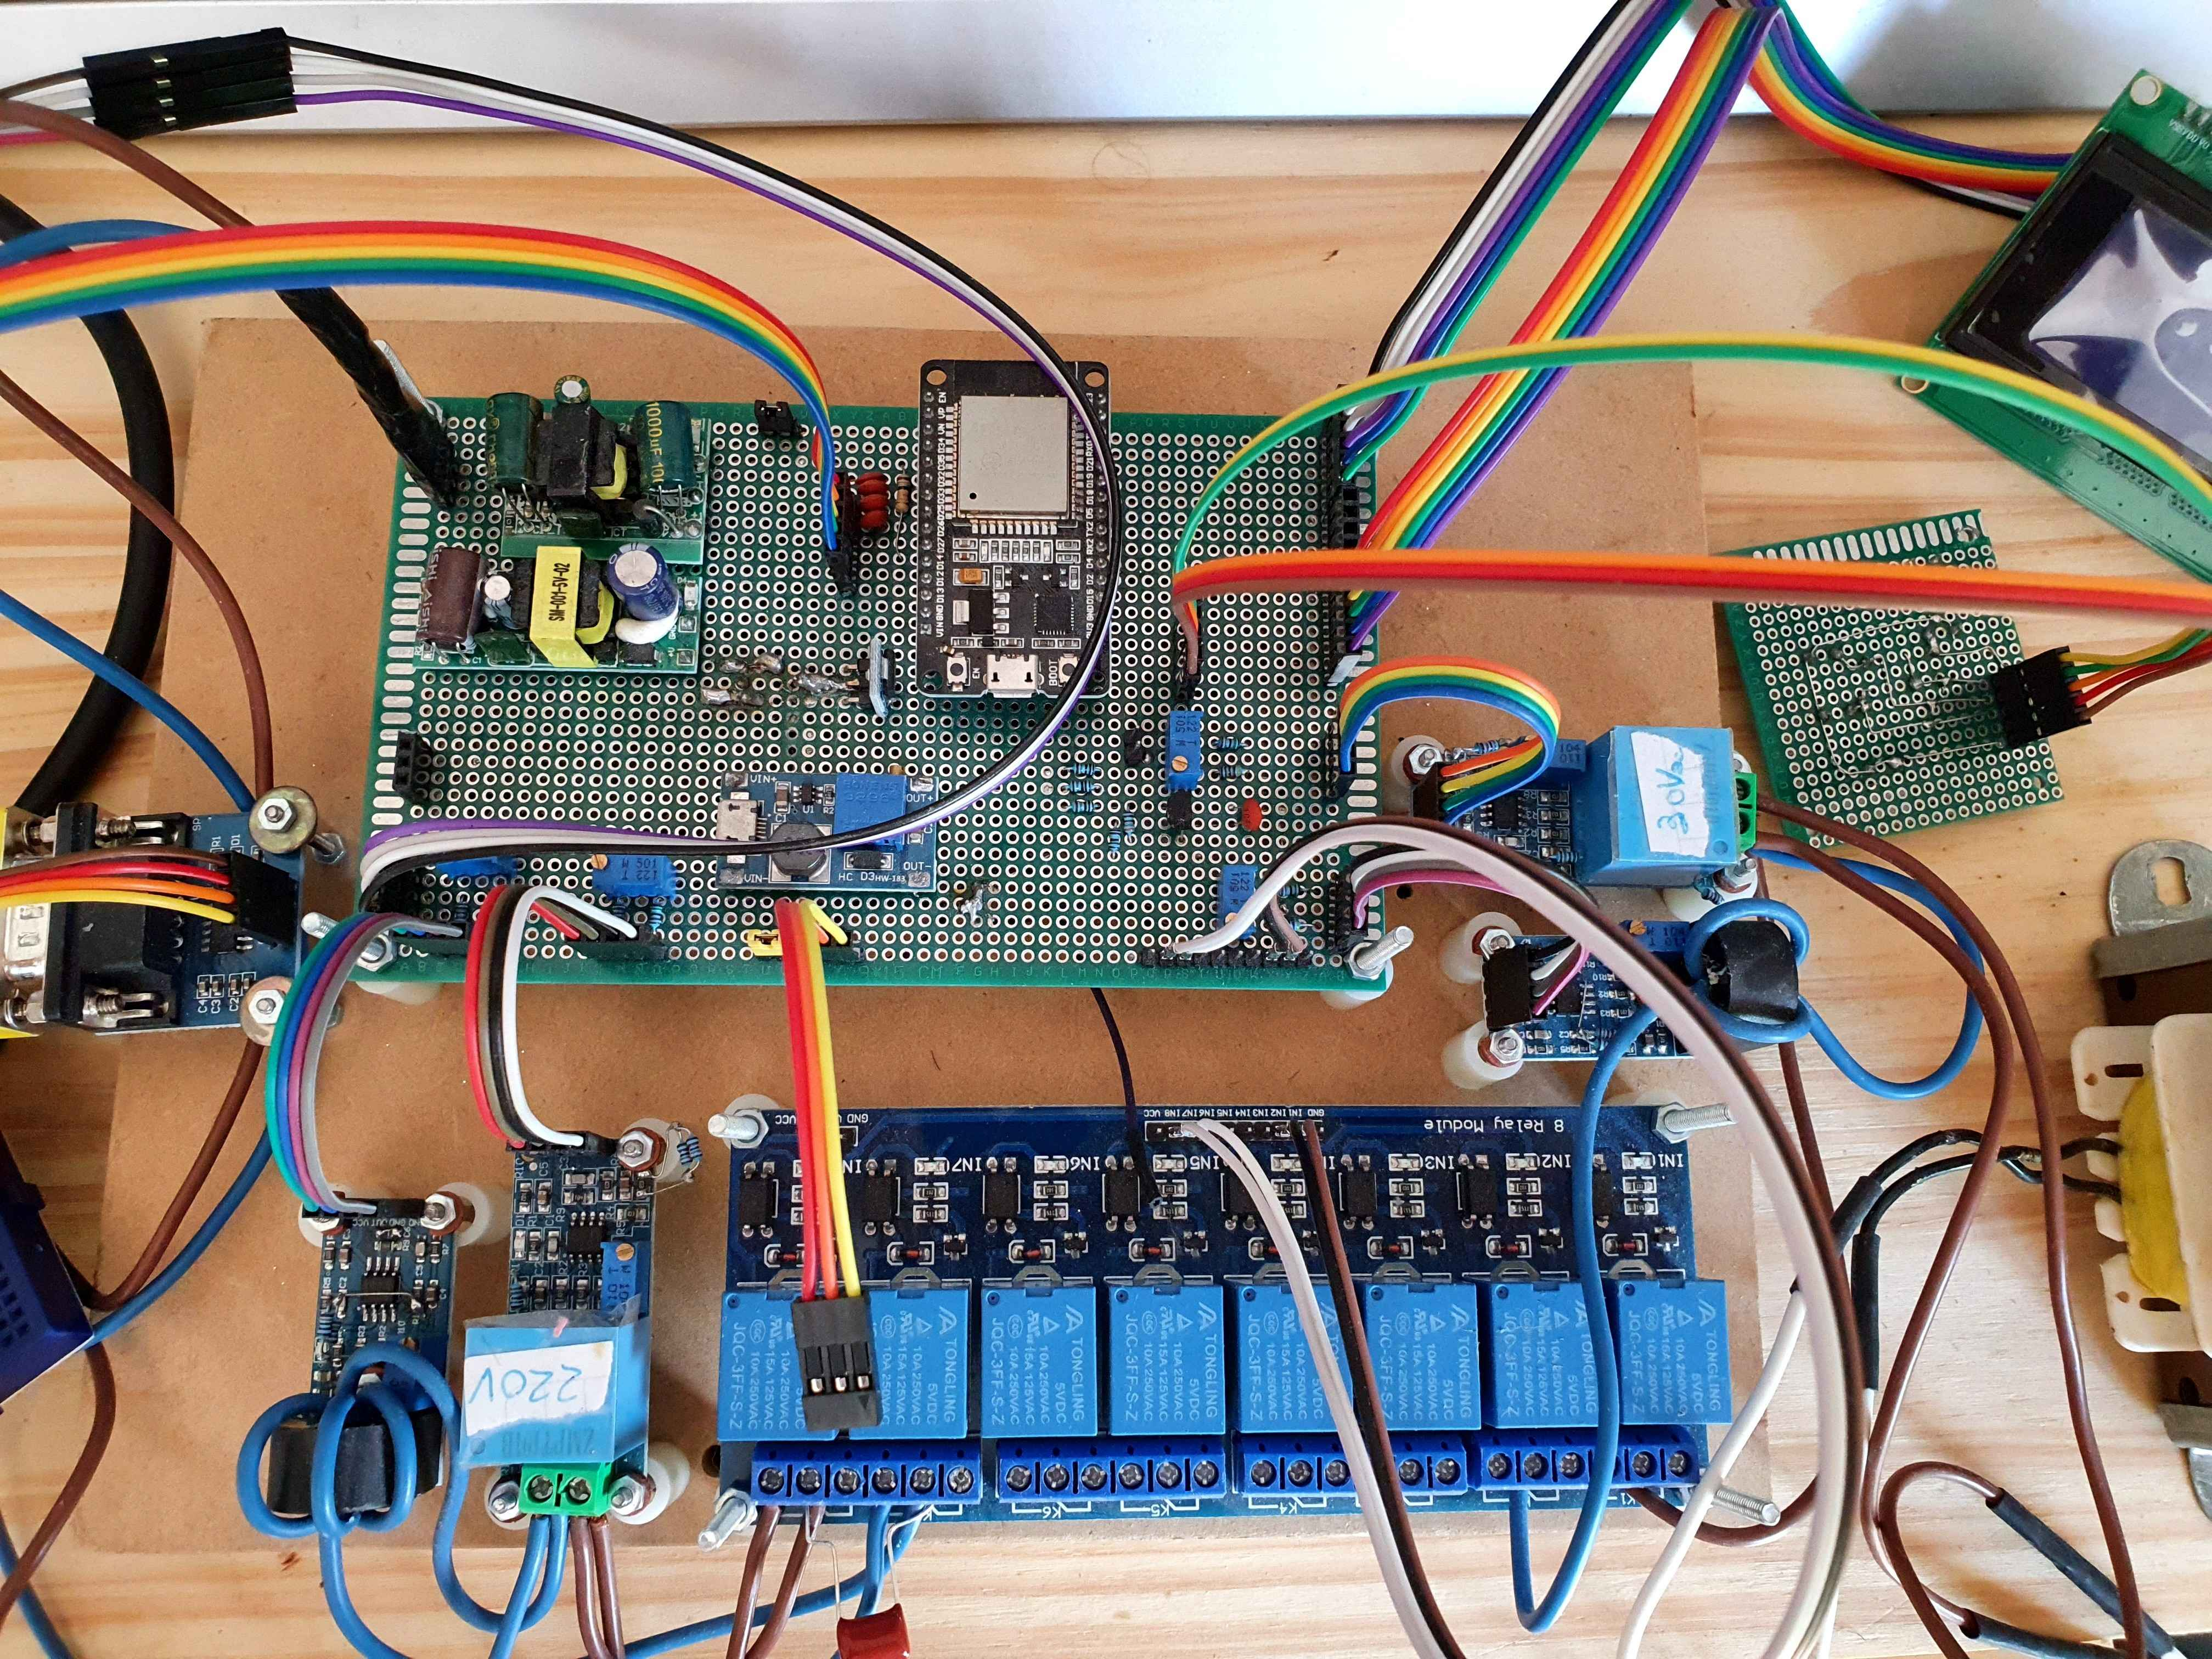
\includegraphics[scale=0.09]{./Figures/madera.jpg}
	\caption{Primera prueba de integración.}
	\label{fig:BaseMadera}
\end{figure}

En esta etapa se realizaron las siguientes pruebas:
\begin{enumerate}
	\item Pruebas del módulo Wi-Fi. Se armaron rutinas básicas de conexión y desconexión y, a través de un \textit{ping} a la IP obtenida por el módulo, se verificó la correcta operación.
	\item Pruebas de las mediciones analógicas. Con la inclusión de la placa universal como interfaz entre los módulos sensores y el kit, se procedió a verificar la lectura de los ADCs dentro del kit.
	\item Pruebas con una impresora de un modelo similar a la adquirida finalmente. Esta impresora fue prestada por el cliente para comprobar la factibilidad de la implementación del protocolo DPL.
\end{enumerate}

Con respecto a las entradas analógicas, se verificó que el período de muestreo fijado sea el esperado. Luego, se evalúo el ruido de la señal digitalizada y se decidió implementar el filtro digital explicado en la sección \ref{subsec:RMS}. Para verificar el filtrado, se procedió a leer el \textit{buffer} de 1024 muestras obtenido del DMA y a leer el mismo \textit{buffer} luego de pasarlo por el filtro digital. En la figura \ref{fig:filtroPrue} se muestra la señal antes y después del filtro y se aprecia la mejora debido al filtrado.

\begin{figure}[htpb]
	\centering
	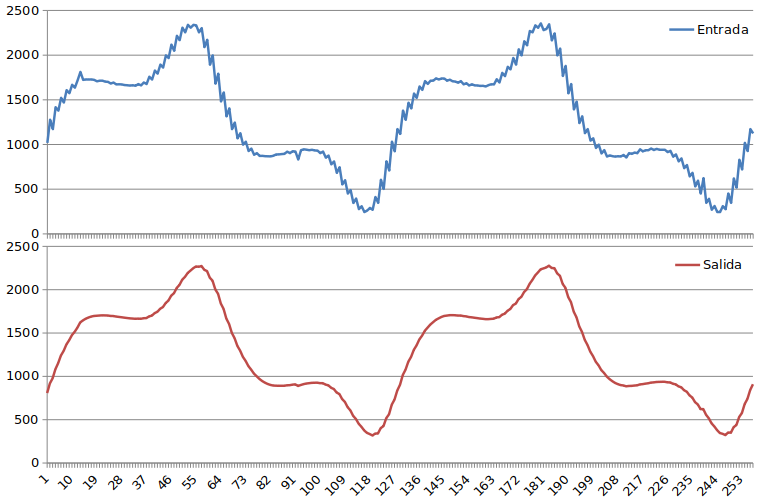
\includegraphics[scale=0.6]{./Figures/filtro.png}
	\caption{Filtro digital aplicado a la medición de corriente .}
	\label{fig:filtroPrue}
\end{figure}

\pagebreak

\section{Ensayos funcionales de integración}
Para los ensayos de integración, se decidió utilizar la metodología \textit{State transition testing} (STT) vista en la asignatura Testing de Software Embebido \citep{STT}. La metodología utilizada establece pasos sistemáticos para las pruebas de sistemas cuya funcionalidad depende de estados, de forma tal, de probar todos los caminos posibles y evitar dejar estados o condiciones sin cubrir. Para cada evento de entrada se debe verificar que:

\begin{enumerate}
	\item Se ejecutan las salidas correctas.
	\item El sistema cambia al estado correcto.
\end{enumerate}

Se tomó la decisión de utilizar esta metodología debido a que el equipo diseñado se comanda por el controlador principal, el cual, está construido sobre una máquina de estados finitos. Basado en lo anterior, tener una buena cobertura de dicha máquina de estados, asegura una buena cobertura del sistema general.

Para implementar la metodología propuesta, se tomaron las sub-máquinas de estados presentadas en la sección \ref{sec:ContSist}. Estas fueron definidas para las etapas de inicialización, de configuración, de caracterización y de reporte. El primer paso fue armar un árbol de transiciones para cada una de ellas, para luego, armar las tablas con los casos de pruebas. En el árbol de transiciones, las transacciones se marcan con un número en la línea de transición entre estados, este número es luego referenciado como ID en la primer columna de las tablas de casos de pruebas. La segunda columna corresponde a las entradas esperadas por parte de la persona encargada de la prueba. En caso de no requerir entrada, porque la transición de estado ocurre en forma automática, se coloca un guion '-' en dicha columna. 

Por otro lado, como salidas, se tiene el \textit{display}, lo enviado o recibido desde el servidor web, el sonido emitido por el \textit{buzzer} y la etiqueta impresa por la impresora. En cada paso, se verifica que dichas interfaces respondan como se espera.

A su vez que se probaron las secuencias definidas por los árboles de transiciones, se validó que dicho comportamiento es consistente con los requerimientos funcionales del sistema presentados en el capítulo \ref{Chapter2}. 

Para los ensayos que se presentan se miden las siguientes variables:
\begin{itemize}
 	\item Tensión en bobinado primario.
	\item Corriente que circula por el bobinado primario.
	\item Tensión en bobinado secundario.
	\item Corriente que circula por el bobinado secundario.
\end{itemize}

En la figura \ref{fig:EnsayoPrimario}, se muestra el banco de pruebas para el bobinado primario y en la figura \ref{fig:EnsayoSecu} se muestra el banco de pruebas para el bobinado secundario. Se puede notar que la medición de corriente carece de sentido cuando el bobinado en cuestión está abierto.

\begin{figure}[htpb]
	\centering
	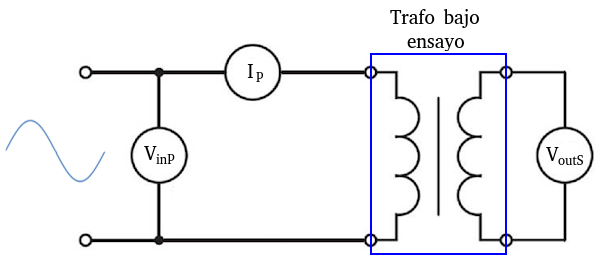
\includegraphics[scale=0.7]{./Figures/EnsayoPrimario.png}
	\caption{Valores medidos en el ensayo de bobinado primario.}
	\label{fig:EnsayoPrimario}
\end{figure}

\begin{figure}[htpb]
	\centering
	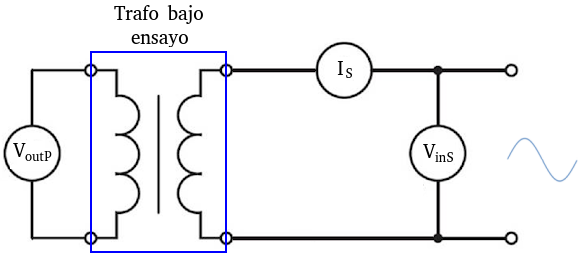
\includegraphics[scale=0.7]{./Figures/EnsayoSecu.png}
	\caption{Valores medidos en el ensayo de bobinado secundario.}
	\label{fig:EnsayoSecu}
\end{figure}

En la tabla \ref{tab:ref_med}, se muestran las convenciones de nombres utilizadas para referenciar los valores medidos de las figuras \ref{fig:EnsayoPrimario} y \ref{fig:EnsayoSecu} en las interfaces del sistema. En la primera columna de la tabla, se muestran los valores medidos y en las columnas subsiguientes, como estos son referenciados en el \textit{display}, en el servidor web y en la etiqueta impresa. 

\begin{table}[htpb]
\centering
\caption[Referencia valores medidos]{Referencia de valores medidos en el \textit{display}, el servidor web y la etiqueta impresa.}
\begin{tabular}{cccc}
\hline
\toprule
\textbf{Variable}                                       & \textbf{\textit{Display}} & \textbf{Servidor web}  & \textbf{Etiqueta} \\
\midrule
\begin{tabular}[c]{@{}c@{}}V$_{inP}$\\ {[}V{]}\end{tabular}  & -       & vinPrimary    & \begin{tabular}[c]{@{}c@{}}VL\\ Se muestra solo si el\\ transformador es rechazado\end{tabular} \\
\begin{tabular}[c]{@{}c@{}}I$_{P}$\\ {[}mA{]}\end{tabular}   & Ip      & iPrimary      & IP \\
\begin{tabular}[c]{@{}c@{}}V$_{outS}$\\ {[}V{]}\end{tabular} & Vs      & voutSecondary & VS \\
\begin{tabular}[c]{@{}c@{}}V$_{inS}$\\ {[}V{]}\end{tabular}  & -       & vinSecondary  & -  \\
\begin{tabular}[c]{@{}c@{}}V$_{outP}$\\ {[}V{]}\end{tabular} & -       & voutPrimary   & -  \\
\begin{tabular}[c]{@{}c@{}}I$_{S}$\\ {[}mA{]}\end{tabular}   & Is      & iSecondary    & IS \\
\bottomrule
\hline
\end{tabular}%
\label{tab:ref_med}
\end{table}

Se puede notar que no todos los valores medidos son mostrados en todas las interfaces. Esto último se debe a una restricción de espacio físico en el \textit{display} y la etiqueta.

\subsection{Pruebas de la etapa de inicialización}

Para la etapa de inicialización, se armó el árbol de transiciones mostrado en la figura \ref{fig:ArTrans_1}.

\begin{figure}[htpb]
	\centering
	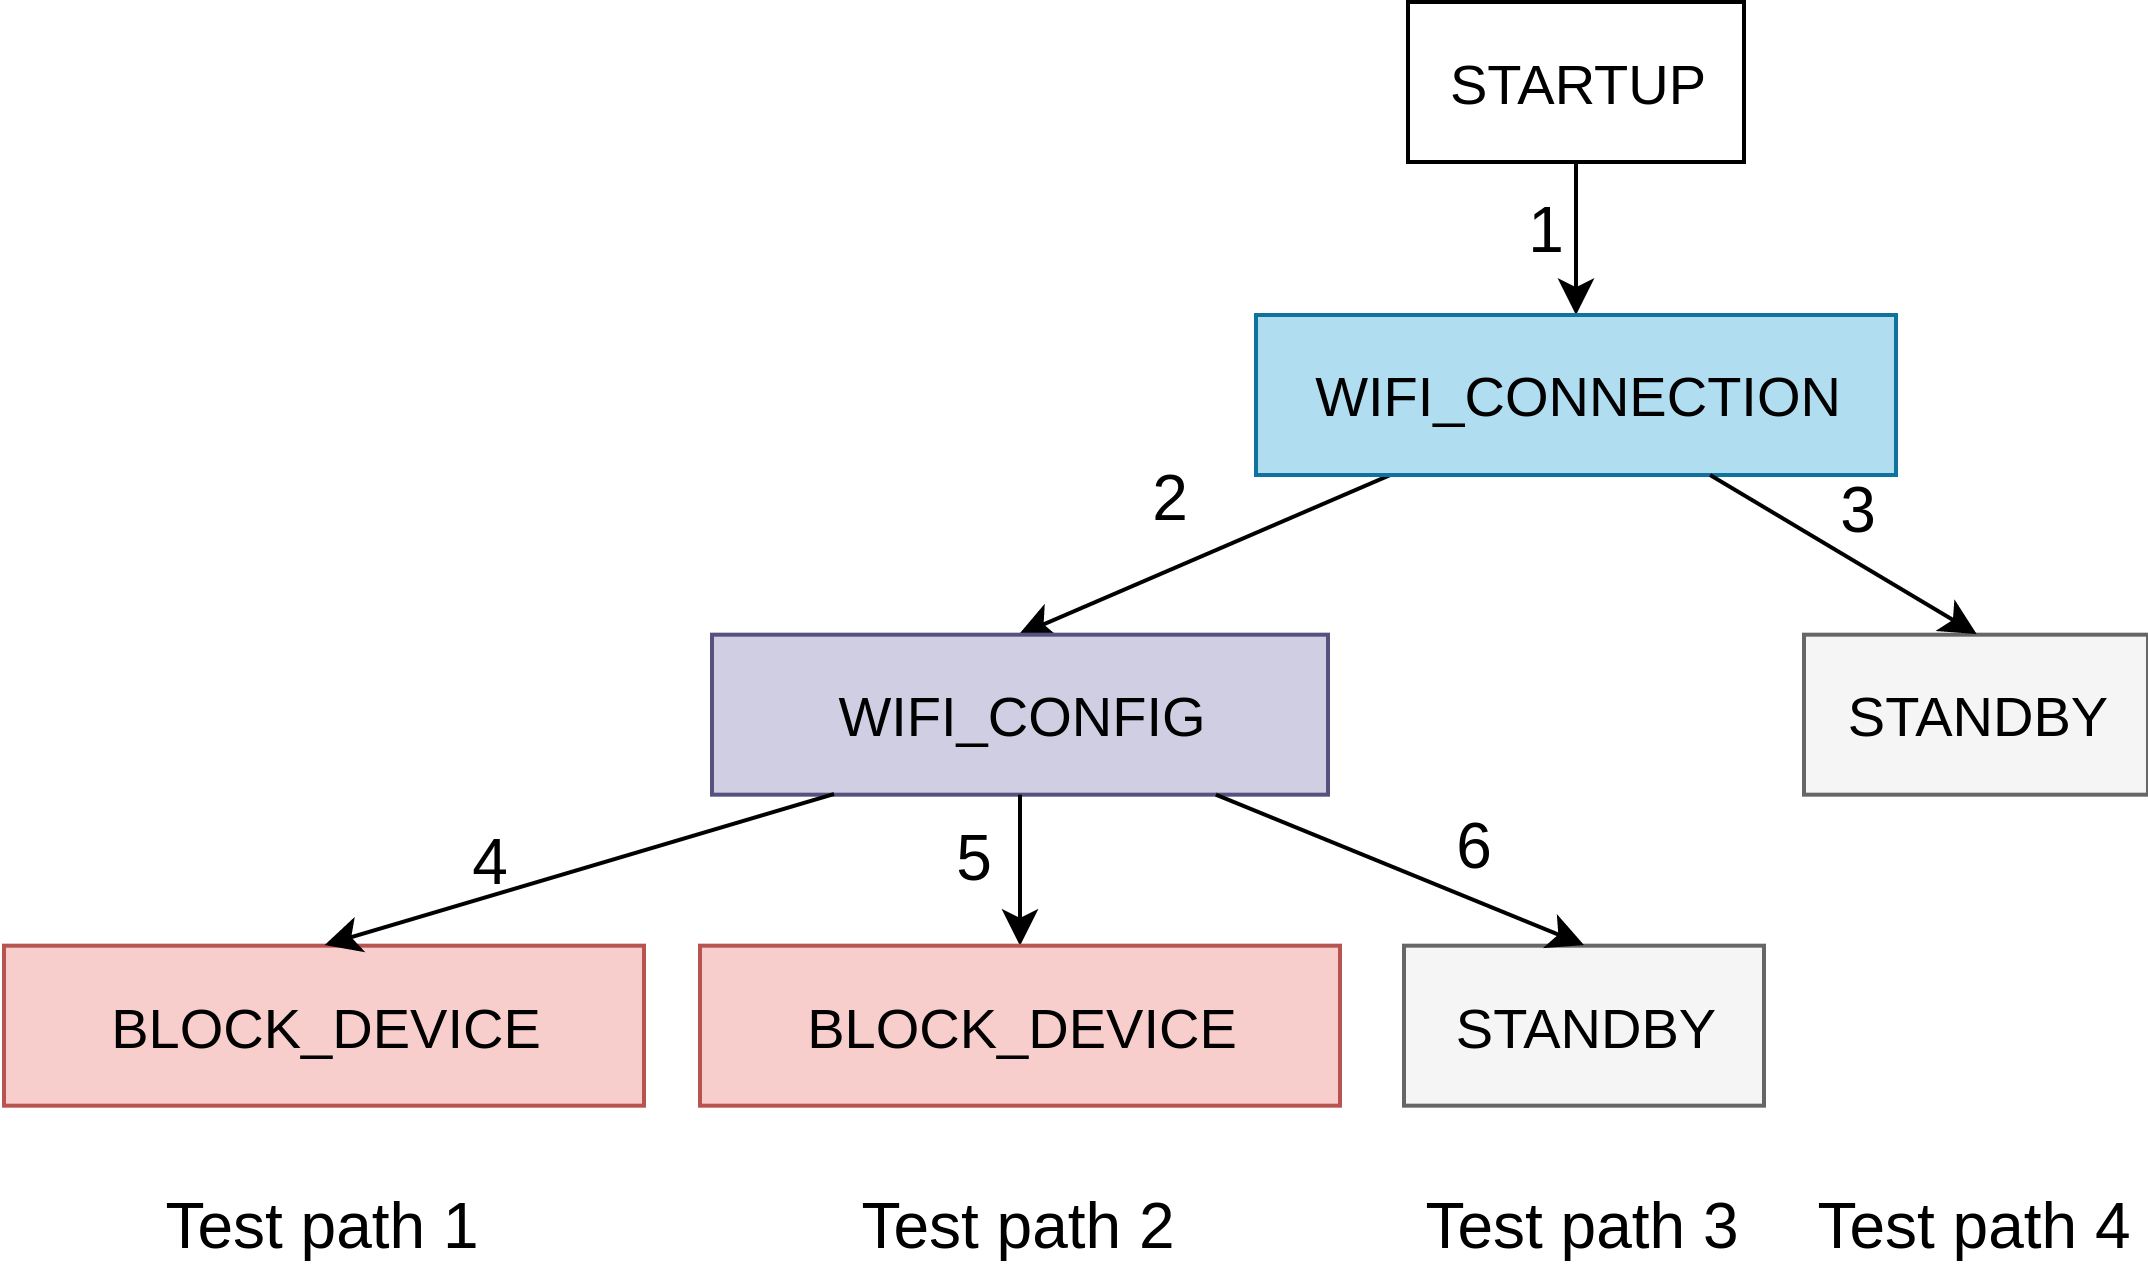
\includegraphics[scale=1]{./Figures/ArTrans_1.png}
	\caption{Árbol de transiciones: etapa de inicialización.}
	\label{fig:ArTrans_1}
\end{figure}

A partir del árbol generado, se obtuvieron cuatro caminos a verificar: \textit{test path} 1 a 4. De estos caminos, se armaron las tablas \ref{tab:pruIni_1} a \ref{tab:pruIni_4} con los casos de pruebas.

Para las pruebas de inicialización, se debe utilizar un equipo sin ningún dato de configuración cargado, de forma tal, de pasar por todos los pasos del árbol de transiciones.

Finalmente, en los casos en que el equipo queda bloqueado, \textit{test path} 1 y 2, se verificó que este no responde a ningún pulsador.

\subsubsection{Prueba del \textit{test path} 1}
\label{subsubsec:pruIni_1}

Condiciones iniciales: 

\begin{enumerate}
	\item Equipo desenergizado.
	\item Impresora encendida y conectada.
\end{enumerate}

En la tabla \ref{tab:pruIni_1}, se muestran los casos de pruebas para el \textit{test path} 1.

\begin{table}[htpb]
\centering
\caption[Prueba de la etapa de inicialización: \textit{test path} 1]{Casos de pruebas para el \textit{test path} 1.}
\resizebox{\textwidth}{!}{%
\begin{tabular}{cclc}
\hline
\toprule
\textbf{ID} & \textbf{Entrada}            & \textbf{Salida}  & \textbf{Estado}           \\
\midrule
-  & Encender el equipo & \begin{tabular}[c]{@{}l@{}}\textit{Display}: mensaje de bienvenida\\ \textit{Buzzer}: sin salida\\ Impresora: sin salida\end{tabular}                                                     & STARTUP          \\ \hline
1  & -                  & \begin{tabular}[c]{@{}l@{}}\textit{Display}: ``Estableciendo conexión WiFi''\\ \textit{Buzzer}: sin salida\\ Impresora: sin salida\end{tabular}                                             & WIFI\_CONNECTION \\ \hline
2  & -                  & \begin{tabular}[c]{@{}l@{}}\textit{Display}: ``Fallo al intentar conectar a WiFi''\\ "Desea configurar WiFi nuevamente?"\\ \textit{Buzzer}: sin salida\\ Impresora: sin salida\end{tabular} & WIFI\_CONFIG     \\ \hline
4  & Pulsar Cancelar    & \begin{tabular}[c]{@{}l@{}}\textit{Display}: ``Sin conexión WiFi Equipo bloqueado''\\ \textit{Buzzer}: sin salida\\ Impresora: sin salida\end{tabular}                                      & BLOCK\_DEVICE \\ 
\bottomrule
\hline
\end{tabular}%
}
\label{tab:pruIni_1}
\end{table}

\pagebreak
Resultado: el ensayo se superó con éxito. En la figura \ref{fig:pruIni_1_res}, se muestran las imágenes obtenidas del \textit{display} para cada paso.

\begin{figure}[!htpb]
     \centering
     \begin{subfigure}[b]{0.4\textwidth}
         \centering
         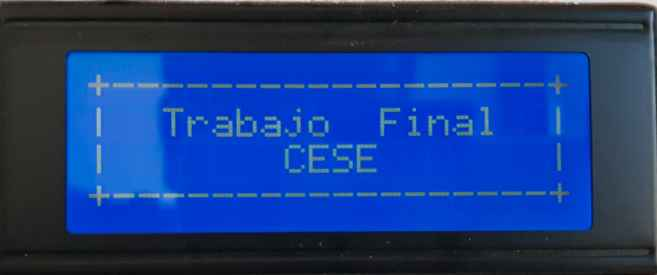
\includegraphics[width=1.1\textwidth]{./Figures/Bienvenida.jpeg}
         \caption{STARTUP.}
         \label{fig:pruIni_1_1}
     \end{subfigure}
     \hfill
     \begin{subfigure}[b]{0.4\textwidth}
         \centering
         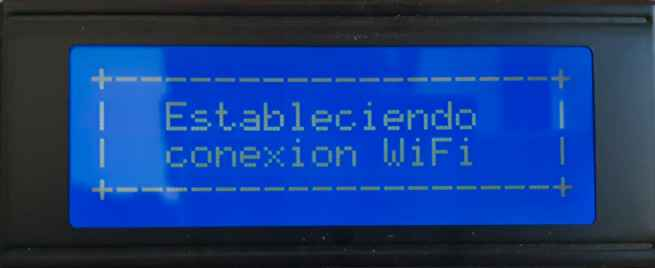
\includegraphics[width=1.1\textwidth]{./Figures/Esta_conex_WiFi.jpeg}
         \caption{WIFI\_CONNECTION}
         \label{fig:pruIni_1_2}
     \end{subfigure}
          \hfill
     \begin{subfigure}[b]{0.4\textwidth}
         \centering
         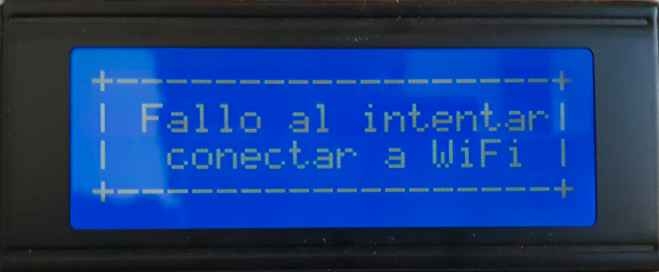
\includegraphics[width=1.1\textwidth]{./Figures/Fallo_con_WiFi.jpeg}
         \caption{WIFI\_CONFIG msg 1.}
         \label{fig:pruIni_1_3}
     \end{subfigure}
          \hfill
     \begin{subfigure}[b]{0.4\textwidth}
         \centering
         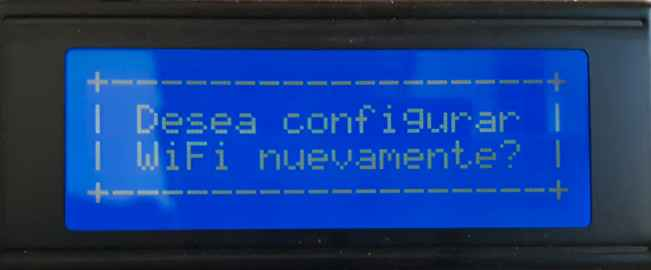
\includegraphics[width=1.1\textwidth]{./Figures/Conf_WiFi_nueva.jpeg}
         \caption{WIFI\_CONFIG msg 2.}
         \label{fig:pruIni_1_4}
     \end{subfigure}
          \hfill
     \begin{subfigure}[b]{0.4\textwidth}
         \centering
         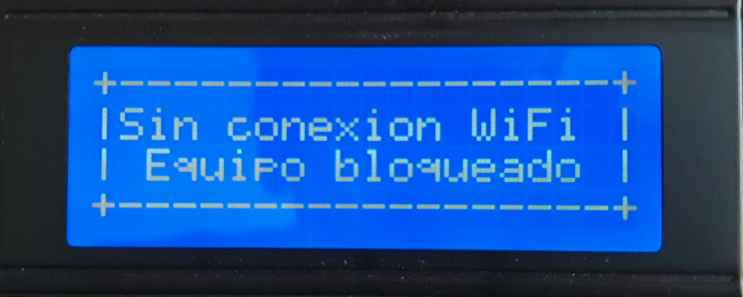
\includegraphics[width=1.1\textwidth]{./Figures/Sin_Conex_WiFi_Eq_Bloq.jpeg}
         \caption{BLOCK\_DEVICE.}
         \label{fig:pruIni_1_5}
     \end{subfigure}
        \caption{Resultado del \textit{test path} 1.}
        \label{fig:pruIni_1_res}
\end{figure}



\subsubsection{Prueba del \textit{test path} 2}
\label{subsubsec:pruIni_2}

Condiciones iniciales: 

\begin{enumerate}
	\item Equipo desenergizado.
	\item Impresora encendida y conectada.
	\item Teléfono móvil con la aplicación ESP-Touch instalada.
\end{enumerate}

En la tabla \ref{tab:pruIni_2}, se muestran los casos de pruebas para el \textit{test path} 2.

\begin{table}[htpb]
\centering
\caption[Prueba de la etapa de inicialización: \textit{test path} 2]{Casos de pruebas para el \textit{test path} 2.}
\resizebox{\textwidth}{!}{%
\begin{tabular}{cclc}
\hline
\toprule
\textbf{ID} & \textbf{Entrada}            & \textbf{Salida}  & \textbf{Estado}           \\
\midrule
-  & Encender el equipo & \begin{tabular}[c]{@{}l@{}}\textit{Display}: mensaje de bienvenida\\ \textit{Buzzer}: sin salida\\ Impresora: sin salida\end{tabular}                                                     & STARTUP          \\ \hline
1  & -                  & \begin{tabular}[c]{@{}l@{}}\textit{Display}: ``Estableciendo conexión WiFi''\\ \textit{Buzzer}: sin salida\\ Impresora: sin salida\end{tabular}                                             & WIFI\_CONNECTION \\ \hline
2  & -                  & \begin{tabular}[c]{@{}l@{}}\textit{Display}: ``Fallo al intentar conectar a WiFi''\\ "Desea configurar WiFi nuevamente?"\\ \textit{Buzzer}: sin salida\\ Impresora: sin salida\end{tabular} & WIFI\_CONFIG     \\ \hline
-  & Pulsar Configurar  & \begin{tabular}[c]{@{}l@{}}\textit{Display}: ``Configure WiFi por SmartConfig''\\ \textit{Buzzer}: sin salida\\ Impresora: sin salida\end{tabular}                                          & \begin{tabular}[c]{@{}c@{}}WIFI\_CONFIG\\ pseudoestado\end{tabular} \\ \hline
5  & \begin{tabular}[c]{@{}c@{}}Insertar datos \\ erróneos\\ en ESP-Touch\end{tabular} & \begin{tabular}[c]{@{}l@{}}\textit{Display}: ``Fallo al conectar por SmartConfig''\\ \textit{Buzzer}: sin salida\\ Impresora: sin salida\end{tabular}                                       & BLOCK\_DEVICE \\ 
\bottomrule
\hline
\end{tabular}%
}
\label{tab:pruIni_2}
\end{table}

Resultado: el ensayo se superó con éxito. En la figura \ref{fig:pruIni_2_res}, se muestran las imágenes obtenidas del \textit{display} para cada paso, se omiten las capturas de los primeros tres pasos ya que son iguales a las del \textit{test path} 1. 
 
\begin{figure}[!htpb]
     \centering
     \begin{subfigure}[b]{0.4\textwidth}
         \centering
         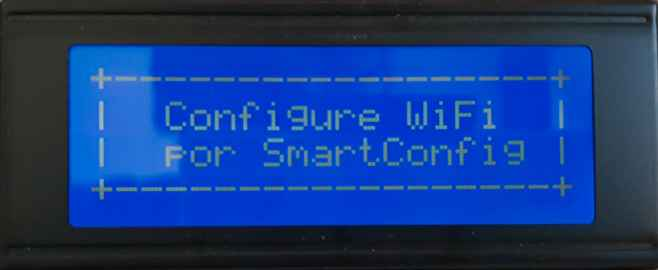
\includegraphics[width=1.1\textwidth]{./Figures/Conf_SmartConf.jpeg}
         \caption{WIFI\_CONFIG msg 4.}
         \label{fig:pruIni_2_1}
     \end{subfigure}
           \hfill
     \begin{subfigure}[b]{0.4\textwidth}
         \centering
         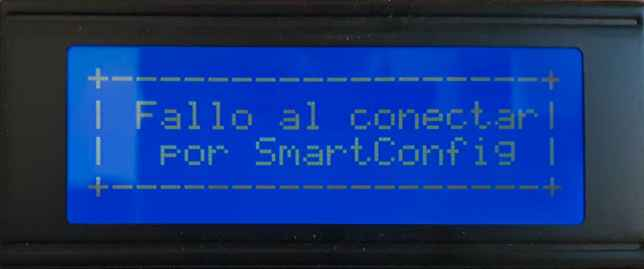
\includegraphics[width=1.1\textwidth]{./Figures/Fallo_SmartConf.jpeg}
         \caption{WIFI\_CONFIG msg 5.}
         \label{fig:pruIni_2_2}
     \end{subfigure}
           \hfill
     \begin{subfigure}[b]{0.4\textwidth}
         \centering
         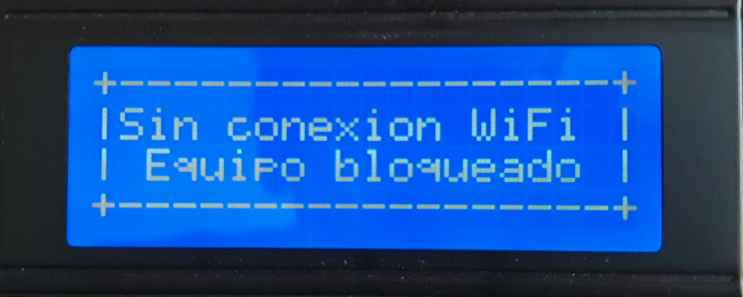
\includegraphics[width=1.1\textwidth]{./Figures/Sin_Conex_WiFi_Eq_Bloq.jpeg}
         \caption{BLOCK\_DEVICE.}
         \label{fig:pruIni_2_3}
     \end{subfigure}
        \caption{Resultado del \textit{test path} 2.}
        \label{fig:pruIni_2_res}
\end{figure}

En la figura \ref{fig:pruIni_2_ESPT}, se muestra una captura de pantalla de la aplicación ESP-Touch donde se observa la falla al intentar transferir las credenciales de Wi-Fi al equipo.

\begin{figure}[htpb]
	\centering
	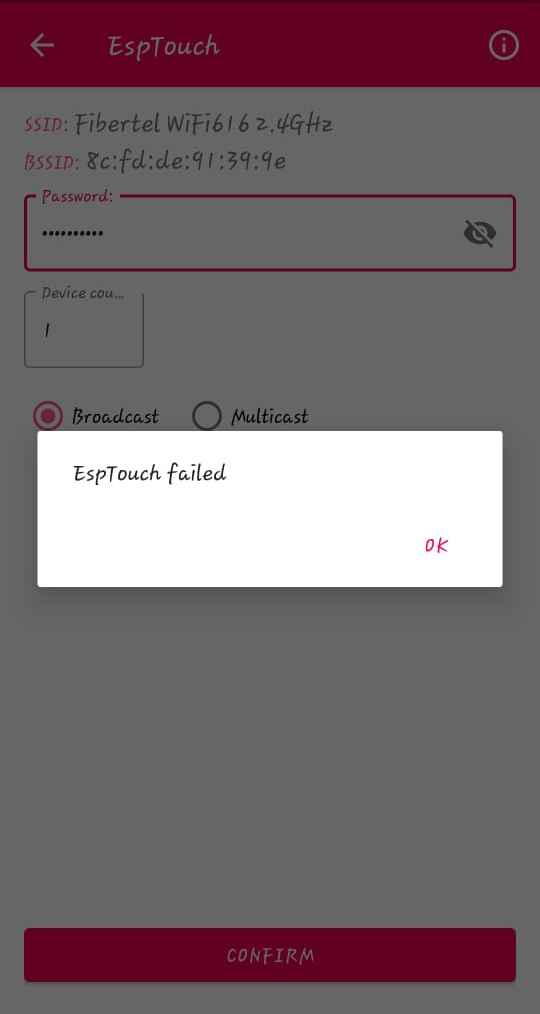
\includegraphics[scale=0.4]{./Figures/ESP_Touch_fail.jpeg}
	\caption{Respuesta de la aplicación ESP-Touch.}
	\label{fig:pruIni_2_ESPT}
\end{figure}

\pagebreak
\subsubsection{Prueba del \textit{test path} 3}
\label{subsubsec:pruIni_3}

Condiciones iniciales: 

\begin{enumerate}
	\item Equipo desenergizado.
	\item Impresora encendida y conectada.
	\item Teléfono móvil con aplicación ESP-Touch instalada.
\end{enumerate}

En la tabla \ref{tab:pruIni_3}, se muestran los casos de pruebas para el \textit{test path} 3.

\begin{table}[htpb]
\centering
\caption[Prueba de la etapa de inicialización: \textit{test path} 3]{Casos de pruebas para el \textit{test path} 3.}
\resizebox{\textwidth}{!}{%
\begin{tabular}{cclc}
\hline
\toprule
\textbf{ID} & \textbf{Entrada}            & \textbf{Salida}  & \textbf{Estado}           \\
\midrule
-  & Encender el equipo & \begin{tabular}[c]{@{}l@{}}\textit{Display}: mensaje de bienvenida\\ \textit{Buzzer}: sin salida\\ Impresora: sin salida\end{tabular}                                                     & STARTUP          \\ \hline
1  & -                  & \begin{tabular}[c]{@{}l@{}}\textit{Display}: ``Estableciendo conexión WiFi''\\ \textit{Buzzer}: sin salida\\ Impresora: sin salida\end{tabular}                                             & WIFI\_CONNECTION \\ \hline
2  & -                  & \begin{tabular}[c]{@{}l@{}}\textit{Display}: ``Fallo al intentar conectar a WiFi''\\ "Desea configurar WiFi nuevamente?"\\ \textit{Buzzer}: sin salida\\ Impresora: sin salida\end{tabular} & WIFI\_CONFIG     \\ \hline
-  & Pulsar Configurar  & \begin{tabular}[c]{@{}l@{}}\textit{Display}: ``Configure WiFi por SmartConfig''\\ \textit{Buzzer}: sin salida\\ Impresora: sin salida\end{tabular}                                          & \begin{tabular}[c]{@{}c@{}}WIFI\_CONFIG\\ pseudoestado\end{tabular} \\ \hline
6  & \begin{tabular}[c]{@{}c@{}}Insertar los datos \\ correctos\\ en ESP-Touch\end{tabular} & \begin{tabular}[c]{@{}l@{}}\textit{Display}: ``Conectado a red WiFi''\\ \textit{Buzzer}: sin salida\\ Impresora: sin salida\end{tabular}  & STANDBY\\ 
\bottomrule
\hline
\end{tabular}%
}
\label{tab:pruIni_3}
\end{table}

\pagebreak
Resultado: el ensayo se superó con éxito. En la figura \ref{fig:pruIni_3_res}, se muestran las imágenes obtenidas del \textit{display} para cada paso, al igual que en la figura anterior, se omiten los primeros tres pasos. 

\begin{figure}[!htpb]
     \centering
     \begin{subfigure}[b]{0.4\textwidth}
         \centering
         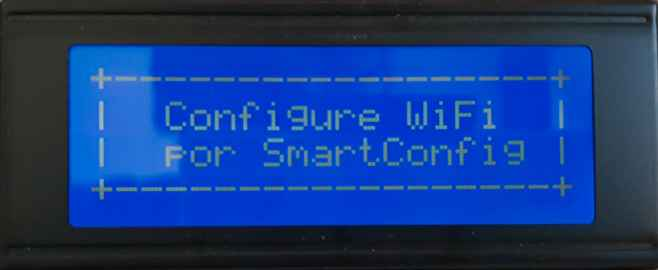
\includegraphics[width=1.1\textwidth]{./Figures/Conf_SmartConf.jpeg}
         \caption{WIFI\_CONFIG msg 4.}
         \label{fig:pruIni_3_1}
     \end{subfigure}
           \hfill
     \begin{subfigure}[b]{0.4\textwidth}
         \centering
         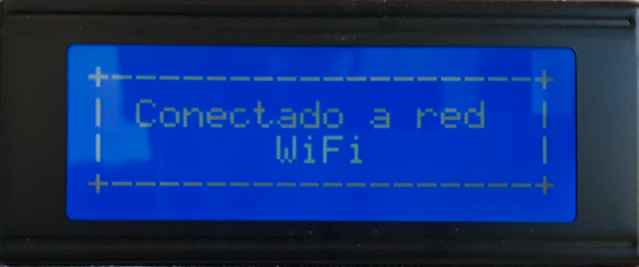
\includegraphics[width=1.1\textwidth]{./Figures/Conect_to_WiFi.jpeg}
         \caption{WIFI\_CONFIG msg 5.}
         \label{fig:pruIni_3_2}
     \end{subfigure}
           \hfill
     \begin{subfigure}[b]{0.4\textwidth}
         \centering
         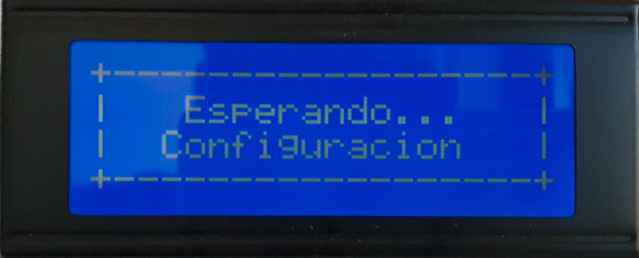
\includegraphics[width=1.1\textwidth]{./Figures/Esp_Conf.jpeg}
         \caption{STANDBY.}
         \label{fig:pruIni_3_3}
     \end{subfigure}
        \caption{Resultado del \textit{test path} 3.}
        \label{fig:pruIni_3_res}
\end{figure}

En la figura \ref{fig:pruIni_3_ESPT_1}, se muestra una captura de pantalla de la aplicación ESP-Touch donde se observa la conexión exitosa a la red Wi-Fi y la IP asignada al equipo en la red. Finalmente, en la figura \ref{fig:pruIni_3_ESPT_2} se muestra que, al conectarse el equipo a la red Wi-Fi, este responde al pedido de \textit{ping} desde el ordenador a la IP indicada por la aplicación ESP-Touch.

\pagebreak

\begin{figure}[htpb]
	\centering
	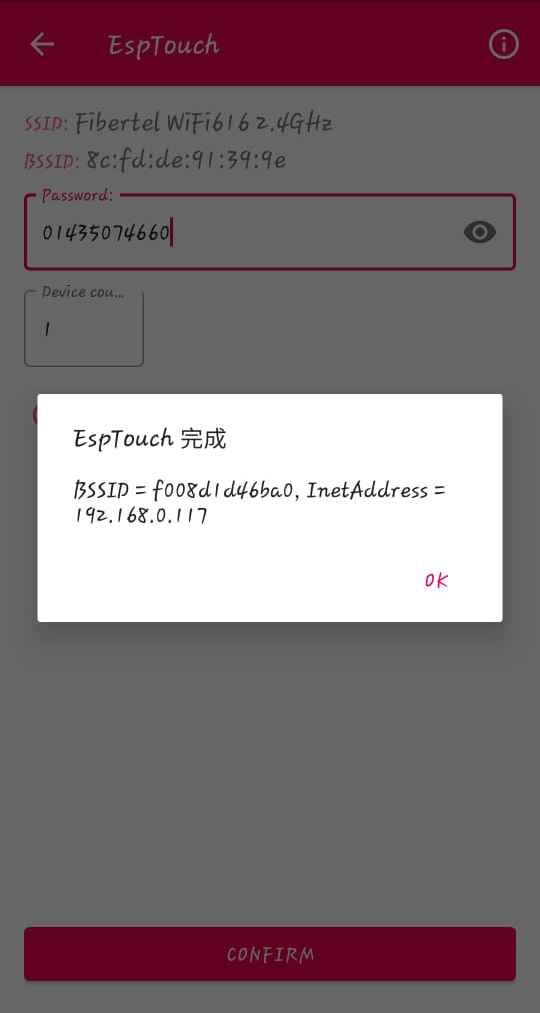
\includegraphics[scale=0.4]{./Figures/ESP_Touch_ok.jpeg}
	\caption{Respuesta de la aplicación ESP-Touch.}
	\label{fig:pruIni_3_ESPT_1}
\end{figure}

\begin{figure}[htpb]
	\centering
	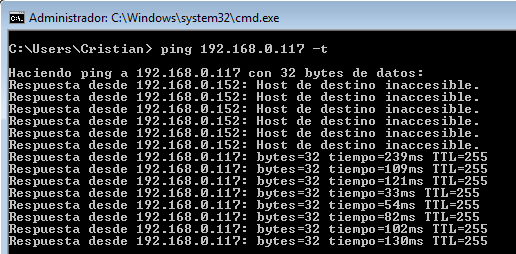
\includegraphics[scale=0.8]{./Figures/ping.png}
	\caption{\textit{Ping} desde la consola a la IP devuelta por ESP-Touch.}
	\label{fig:pruIni_3_ESPT_2}
\end{figure}

\subsubsection{Prueba del \textit{test path} 4}
\label{subsubsec:pruIni_4}

Condiciones iniciales: 

\begin{enumerate}
	\item Equipo desenergizado.
	\item Impresora encendida y conectada.
\end{enumerate}


En la tabla \ref{tab:pruIni_4}, se muestran los casos de pruebas para el \textit{test path} 4.

\begin{table}[htpb]
\centering
\caption[Prueba de la etapa de inicialización: \textit{test path} 4]{Casos de pruebas para el \textit{test path} 4.}
\resizebox{\textwidth}{!}{%
\begin{tabular}{cclc}
\hline
\toprule
\textbf{ID} & \textbf{Entrada}            & \textbf{Salida}  & \textbf{Estado}           \\
\midrule
-  & Encender el equipo & \begin{tabular}[c]{@{}l@{}}\textit{Display}: mensaje de bienvenida\\ \textit{Buzzer}: sin salida\\ Impresora: sin salida\end{tabular}                                                     & STARTUP          \\ \hline
1  & -                  & \begin{tabular}[c]{@{}l@{}}\textit{Display}: ``Estableciendo conexión WiFi''\\ \textit{Buzzer}: sin salida\\ Impresora: sin salida\end{tabular}                                             & WIFI\_CONNECTION \\ \hline
3  & - & \begin{tabular}[c]{@{}l@{}}\textit{Display}: ``Esperando... Configuración''\\ \textit{Buzzer}: sin salida\\ Impresora: sin salida\end{tabular}  & STANDBY\\ 
\bottomrule
\hline
\end{tabular}%
}
\label{tab:pruIni_4}
\end{table}

\pagebreak

Resultado: el ensayo se superó con éxito. En la figura \ref{fig:pruIni_4_res}, se muestran las imágenes obtenidas del \textit{display} para cada paso. En este caso, el equipo no requiere interacción con el operador ya que, las credenciales de Wi-Fi fueron correctamente configuradas en el paso anterior y se guardaron en la memoria no volátil del equipo.

\begin{figure}[!htpb]
     \centering
     \begin{subfigure}[b]{0.4\textwidth}
         \centering
         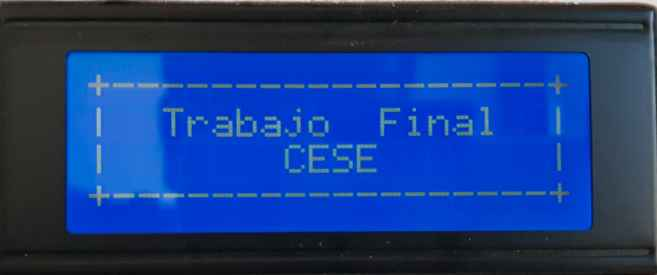
\includegraphics[width=1.1\textwidth]{./Figures/Bienvenida.jpeg}
         \caption{STARTUP.}
         \label{fig:pruIni_4_1}
     \end{subfigure}
           \hfill
     \begin{subfigure}[b]{0.4\textwidth}
         \centering
         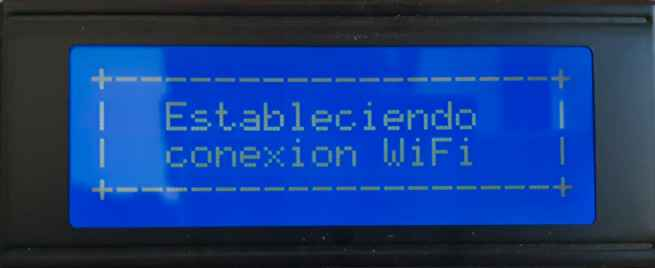
\includegraphics[width=1.1\textwidth]{./Figures/Esta_conex_WiFi.jpeg}
         \caption{WIFI\_CONNECTION}
         \label{fig:pruIni_4_2}
     \end{subfigure}
           \hfill
     \begin{subfigure}[b]{0.4\textwidth}
         \centering
         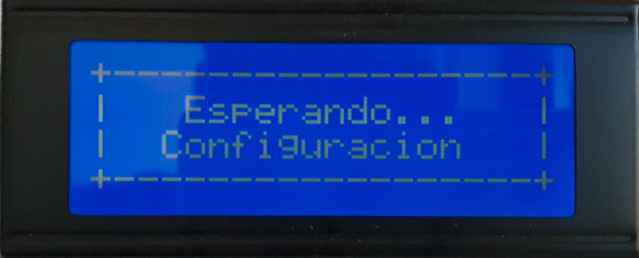
\includegraphics[width=1.1\textwidth]{./Figures/Esp_Conf.jpeg}
         \caption{STANDBY.}
         \label{fig:pruIni_4_3}
     \end{subfigure}
        \caption{Resultado del \textit{test path} 4.}
        \label{fig:pruIni_4_res}
\end{figure}

\subsection{Pruebas de la etapa de configuración}

Para la etapa de configuración, se armó el árbol de transiciones mostrado en la figura \ref{fig:ArTrans_2}. A partir de este, se obtuvieron tres caminos a verificar: \textit{test path} 5 a 7, de los cuales, surgen las tablas \ref{tab:pruConf_5} a \ref{tab:pruConf_7} con los casos de pruebas.

\begin{figure}[htpb]
	\centering
	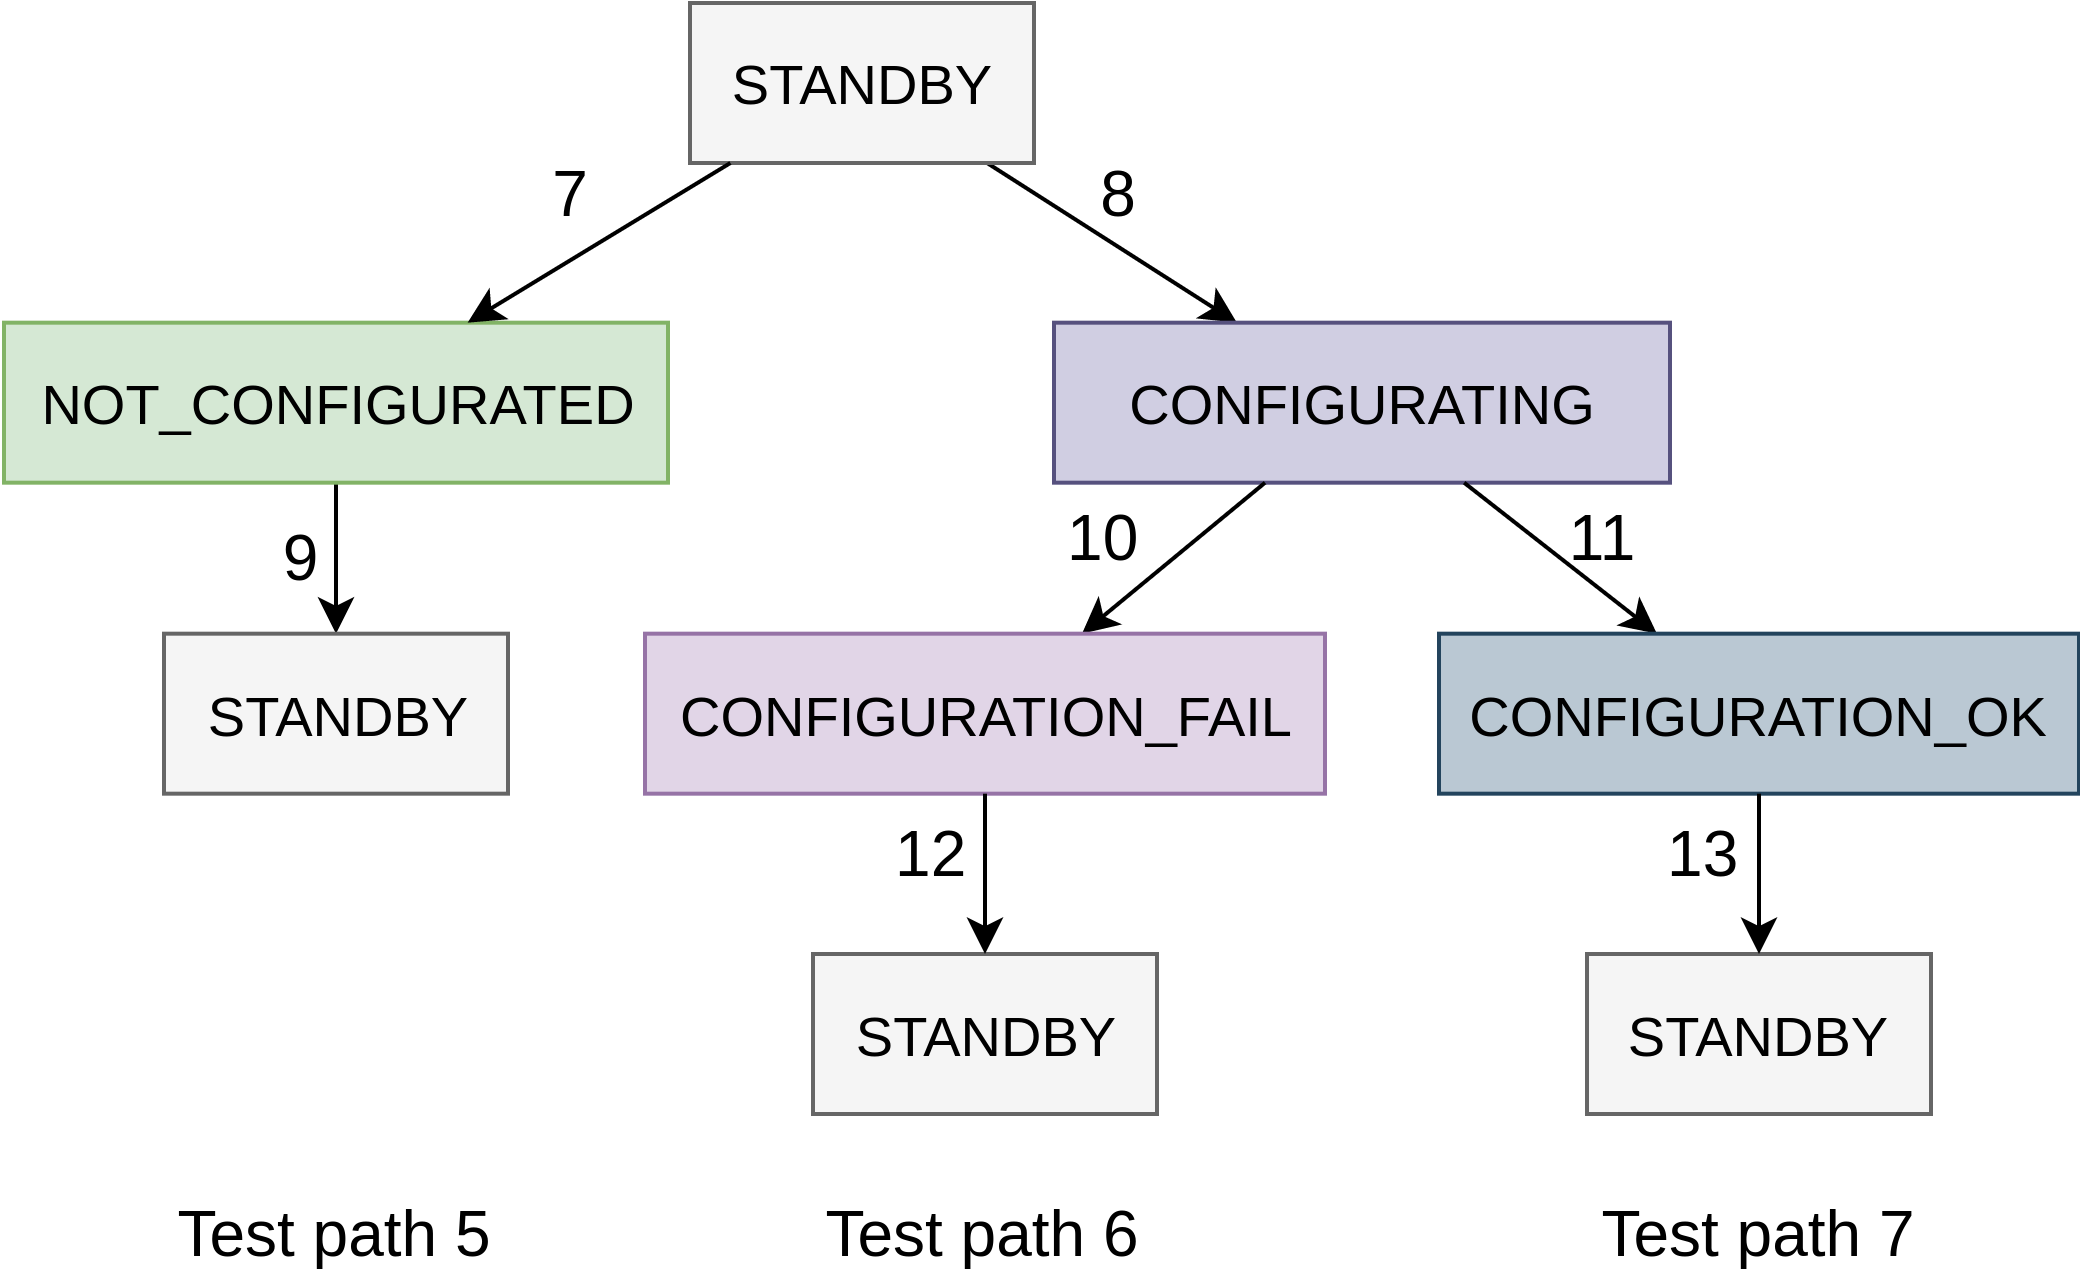
\includegraphics[scale=1]{./Figures/ArTrans_2.png}
	\caption{Árbol de transiciones: etapa de configuración.}
	\label{fig:ArTrans_2}
\end{figure}

Para las pruebas de configuración, se parte siempre del estado STANDBY, por lo tanto, se tiene que superar el \textit{test path} 4 del estado de inicialización para poder comenzar las pruebas de esta etapa.

\pagebreak

A partir de estos ensayos, se pudieron validar los requerimientos: 
\begin{itemize}
\item Requerimientos 1 y 2 de la sección \ref{subsec:ReqFun}.
\item Requerimientos 1 y 2 de la sección \ref{subsec:ReqCom}.
\item Requerimientos 1.a y 2.a de la sección \ref{subsec:ReqUsu}.
\end{itemize}

\subsubsection{Prueba del \textit{test path} 5}
\label{subsubsec:pruConf_5}

Condiciones iniciales: 

\begin{enumerate}
	\item Equipo energizado y \textit{test path} 4 corrido.
	\item Impresora encendida y conectada.
\end{enumerate}

En la tabla \ref{tab:pruConf_5}, se muestran los casos de pruebas para el \textit{test path} 5.

\begin{table}[htpb]
\centering
\caption[Prueba de la etapa de configuración: \textit{test path} 5]{Casos de pruebas para el \textit{test path} 5.}
\resizebox{\textwidth}{!}{%
\begin{tabular}{cclc}
\hline
\toprule
\textbf{ID} & \textbf{Entrada}            & \textbf{Salida}  & \textbf{Estado}           \\
\midrule
-  & -        & \begin{tabular}[c]{@{}l@{}}\textit{Display}: ``Esperando... Configuración''\\ \textit{Buzzer}: sin salida\\ Impresora: sin salida\end{tabular} & STANDBY           \\ \hline
7  & Pulsar Testear & \begin{tabular}[c]{@{}l@{}}\textit{Display}: ``Equipo no configurado''\\ \textit{Buzzer}: sin salida\\ Impresora: sin salida\end{tabular}      & NOT\_CONFIGURATED \\ \hline
9  & -        & \begin{tabular}[c]{@{}l@{}}\textit{Display}: ``Esperando... Configuración''\\ \textit{Buzzer}: sin salida\\ Impresora: sin salida\end{tabular} & STANDBY          
\\ 
\bottomrule
\hline
\end{tabular}%
}
\label{tab:pruConf_5}
\end{table}

Resultado: el ensayo se superó con éxito. En la figura \ref{fig:pruConf_5_res}, se muestran las imágenes obtenidas del \textit{display} para cada paso.

\begin{figure}[!htpb]
     \centering
     \begin{subfigure}[b]{0.4\textwidth}
         \centering
         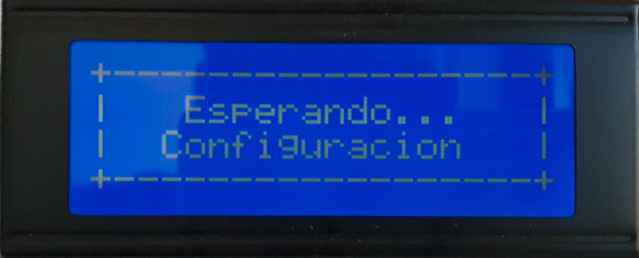
\includegraphics[width=1.1\textwidth]{./Figures/Esp_Conf.jpeg}
         \caption{STANDBY.}
         \label{fig:pruConf_5_1}
     \end{subfigure}
           \hfill
     \begin{subfigure}[b]{0.4\textwidth}
         \centering
         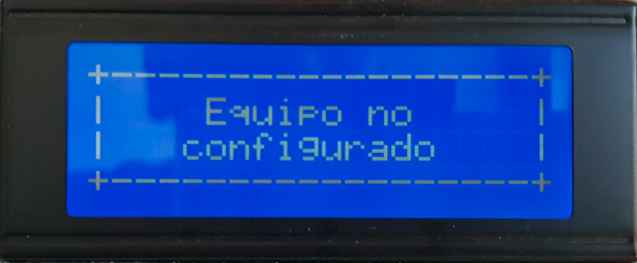
\includegraphics[width=1.1\textwidth]{./Figures/Eq_no_conf.jpeg}
         \caption{NOT\_CONFIGURATED.}
         \label{fig:pruConf_5_2}
     \end{subfigure}
           \hfill
     \begin{subfigure}[b]{0.4\textwidth}
         \centering
         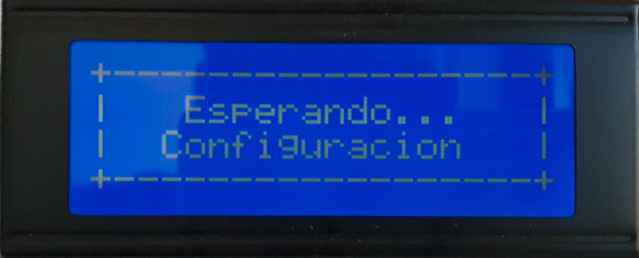
\includegraphics[width=1.1\textwidth]{./Figures/Esp_Conf.jpeg}
         \caption{STANDBY.}
         \label{fig:pruConf_5_3}
     \end{subfigure}
        \caption{Resultado del \textit{test path} 5.}
        \label{fig:pruConf_5_res}
\end{figure}

\pagebreak

\subsubsection{Prueba del \textit{test path} 6}
\label{subsubsec:pruConf_6}

Condiciones iniciales: 

\begin{enumerate}
	\item Equipo energizado y \textit{test path} 4 corrido.
	\item Impresora encendida y conectada.
	\item Servidor web no disponible. Se le pidió al cliente que detenga el servidor web para llevar a cabo la prueba.
\end{enumerate}

En la tabla \ref{tab:pruConf_6}, se muestran los casos de pruebas para el \textit{test path} 6.

\begin{table}[htpb]
\centering
\caption[Prueba de la etapa de configuración: \textit{test path} 6]{Casos de pruebas para el \textit{test path} 6.}
\resizebox{\textwidth}{!}{%
\begin{tabular}{cclc}
\hline
\toprule
\textbf{ID} & \textbf{Entrada}            & \textbf{Salida}  & \textbf{Estado}           \\
\midrule
-  & -        & \begin{tabular}[c]{@{}l@{}}\textit{Display}: ``Esperando... Configuración''\\ \textit{Buzzer}: sin salida\\ Impresora: sin salida\end{tabular} & STANDBY           \\ \hline
8  & Pulsar Configurar                                                              & \begin{tabular}[c]{@{}l@{}}\textit{Display}: ``Configurando Espere...''\\ \textit{Buzzer}: sin salida\\ Impresora: sin salida\end{tabular}     & CONFIGURATING       \\ \hline
10 & \begin{tabular}[c]{@{}c@{}}Servidor web\\no disponible\end{tabular} & \begin{tabular}[c]{@{}l@{}}\textit{Display}: ``Falla en configuración''\\ \textit{Buzzer}: sin salida\\ Impresora: sin salida\end{tabular}     & CONFIGURATION\_FAIL \\ \hline
12  & -        & \begin{tabular}[c]{@{}l@{}}\textit{Display}: ``Esperando... Configuración''\\ \textit{Buzzer}: sin salida\\ Impresora: sin salida\end{tabular} & STANDBY          
\\ 
\bottomrule
\hline
\end{tabular}%
}
\label{tab:pruConf_6}
\end{table}

Resultado: el ensayo se superó con éxito. En la figura \ref{fig:pruConf_6_res}, se muestran las imágenes obtenidas del \textit{display} para cada paso.

\begin{figure}[!htpb]
     \centering
     \begin{subfigure}[b]{0.4\textwidth}
         \centering
         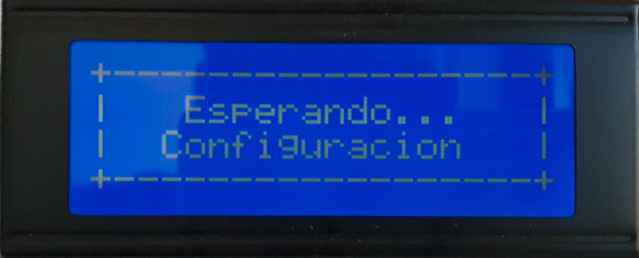
\includegraphics[width=1.1\textwidth]{./Figures/Esp_Conf.jpeg}
         \caption{STANDBY.}
         \label{fig:pruConf_6_1}
     \end{subfigure}
           \hfill
     \begin{subfigure}[b]{0.4\textwidth}
         \centering
         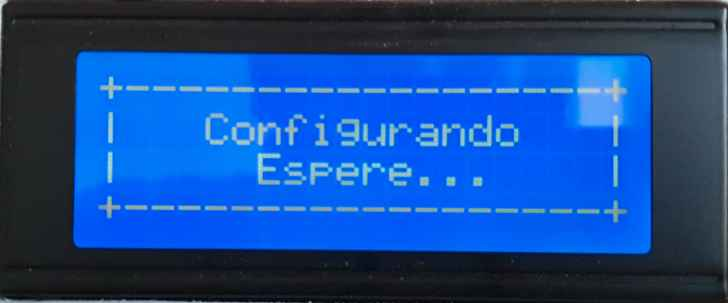
\includegraphics[width=1.1\textwidth]{./Figures/Conf_esp.jpeg}
         \caption{CONFIGURATING.}
         \label{fig:pruConf_6_2}
     \end{subfigure}
           \hfill
     \begin{subfigure}[b]{0.4\textwidth}
         \centering
         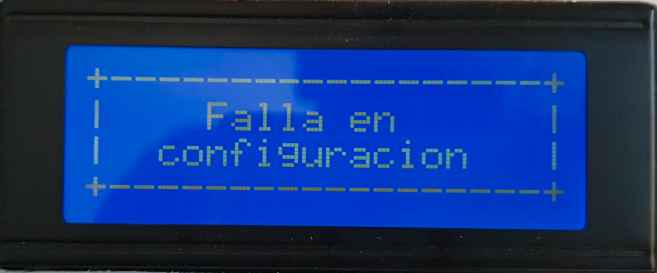
\includegraphics[width=1.1\textwidth]{./Figures/Falla_conf.jpeg}
         \caption{CONFIGURATION\_FAIL.}
         \label{fig:pruConf_6_3}
     \end{subfigure}
           \hfill
     \begin{subfigure}[b]{0.4\textwidth}
         \centering
         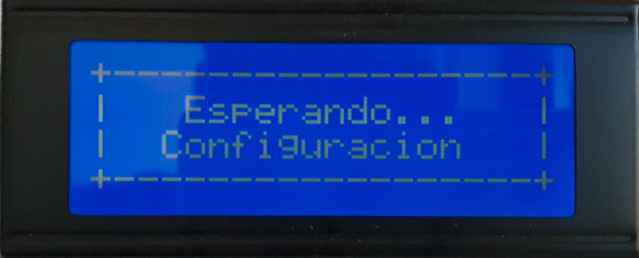
\includegraphics[width=1.1\textwidth]{./Figures/Esp_Conf.jpeg}
         \caption{STANDBY.}
         \label{fig:pruConf_6_4}
     \end{subfigure}
        \caption{Resultado del \textit{test path} 6.}
        \label{fig:pruConf_6_res}
\end{figure}

\pagebreak

\subsubsection{Prueba del \textit{test path} 7}
\label{subsubsec:pruConf_7}

Condiciones iniciales: 

\begin{enumerate}
	\item Equipo energizado y \textit{test path} 4 corrido.
	\item Impresora encendida y conectada.
	\item Servidor web en condiciones operativas y con datos validos. Los datos cargados en el servidor se muestran en la figura \ref{fig:serv_web_conf}. Para obtener esta información se envío un comando GET de HTTP al servidor web a través del explorador Firefox. Los datos se encuentran en formato JSON.
\end{enumerate}

\begin{figure}[htpb]
	\centering
	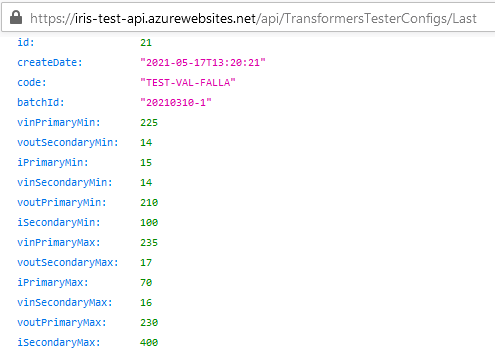
\includegraphics[scale=1]{./Figures/serv_web_falla_conf.png}
	\caption{Datos de configuración en el servidor web.}
	\label{fig:serv_web_conf}
\end{figure}

En la tabla \ref{tab:pruConf_7}, se muestran los casos de pruebas para el \textit{test path} 7.

\begin{table}[htpb]
\centering
\caption[Prueba de la etapa de configuración: \textit{test path} 7]{Casos de pruebas para el \textit{test path} 7.}
\resizebox{\textwidth}{!}{%
\begin{tabular}{cclc}
\hline
\toprule
\textbf{ID} & \textbf{Entrada}            & \textbf{Salida}  & \textbf{Estado}           \\
\midrule
-  & -        & \begin{tabular}[c]{@{}l@{}}\textit{Display}: ``Esperando... Configuración''\\ \textit{Buzzer}: sin salida\\ Impresora: sin salida\end{tabular} & STANDBY           \\ \hline
8  & Pulsar Configurar                                                              & \begin{tabular}[c]{@{}l@{}}\textit{Display}: ``Configurando Espere...''\\ \textit{Buzzer}: sin salida\\ Impresora: sin salida\end{tabular}     & CONFIGURATING       \\ \hline
11 & \begin{tabular}[c]{@{}c@{}}Servidor web\\ con datos \\ válidos\end{tabular} & \begin{tabular}[c]{@{}l@{}}\textit{Display}: mostrar los datos del servidor web\\ \textit{Buzzer}: sin salida\\ Impresora: sin salida\end{tabular}     & CONFIGURATION\_OK \\ \hline
13  & -        & \begin{tabular}[c]{@{}l@{}}\textit{Display}: mostrar los datos del servidor web\\ \textit{Buzzer}: sin salida\\ Impresora: sin salida\end{tabular} & STANDBY          
\\ 
\bottomrule
\hline
\end{tabular}%
}
\label{tab:pruConf_7}
\end{table}

Resultado: el ensayo se superó con éxito. En la figura \ref{fig:pruConf_7_res}, se muestran las imágenes obtenidas del \textit{display} para cada paso. 

\begin{figure}[!htpb]
     \centering
     \begin{subfigure}[b]{0.4\textwidth}
         \centering
         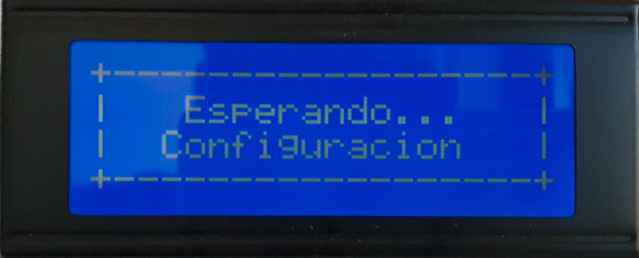
\includegraphics[width=1.1\textwidth]{./Figures/Esp_Conf.jpeg}
         \caption{STANDBY.}
         \label{fig:pruConf_7_1}
     \end{subfigure}
           \hfill
     \begin{subfigure}[b]{0.4\textwidth}
         \centering
         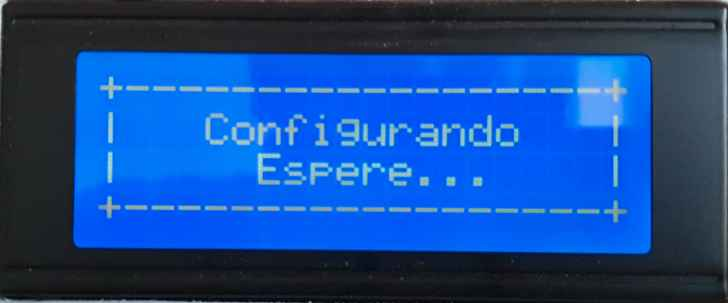
\includegraphics[width=1.1\textwidth]{./Figures/Conf_esp.jpeg}
         \caption{CONFIGURATING.}
         \label{fig:pruConf_7_2}
     \end{subfigure}
           \hfill
     \begin{subfigure}[b]{0.4\textwidth}
         \centering
         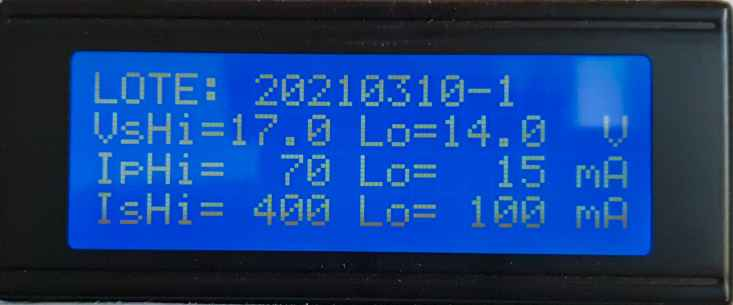
\includegraphics[width=1.1\textwidth]{./Figures/pru_fail.jpeg}
         \caption{CONFIGURATION\_OK.}
         \label{fig:pruConf_7_3}
     \end{subfigure}
           \hfill
     \begin{subfigure}[b]{0.4\textwidth}
         \centering
         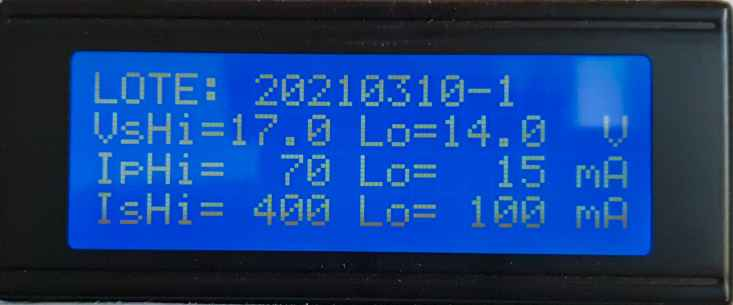
\includegraphics[width=1.1\textwidth]{./Figures/pru_fail.jpeg}
         \caption{STANDBY.}
         \label{fig:pruConf_7_4}
     \end{subfigure}
        \caption{Resultado del \textit{test path} 7.}
        \label{fig:pruConf_7_res}
\end{figure}

En las subfiguras \ref{fig:pruConf_7_3} y \ref{fig:pruConf_7_4}, correspondientes a los pasos 11 y 13, se muestran, en el \textit{display}, algunos de los datos obtenidos del servidor web. Se verificó que los datos de las subfiguras coincidan con los datos almacenados en el servidor web que se presentaron en la figura \ref{fig:serv_web_conf}. Para realizar esta comparación se debe tener en cuenta las referencias mostradas en la tabla \ref{tab:ref_med}.

\subsection{Pruebas de la etapa de caracterización}

Para la etapa de caracterización, se armó el árbol de transiciones mostrado en la figura \ref{fig:ArTrans_3}. A partir de este, se obtuvieron cuatro caminos a verificar: \textit{test path} 8 a 11, de los cuales, surgen las tablas \ref{tab:pruCarac_8} a \ref{tab:pruCarac_11} con los casos de pruebas.

\begin{figure}[htpb]
	\centering
	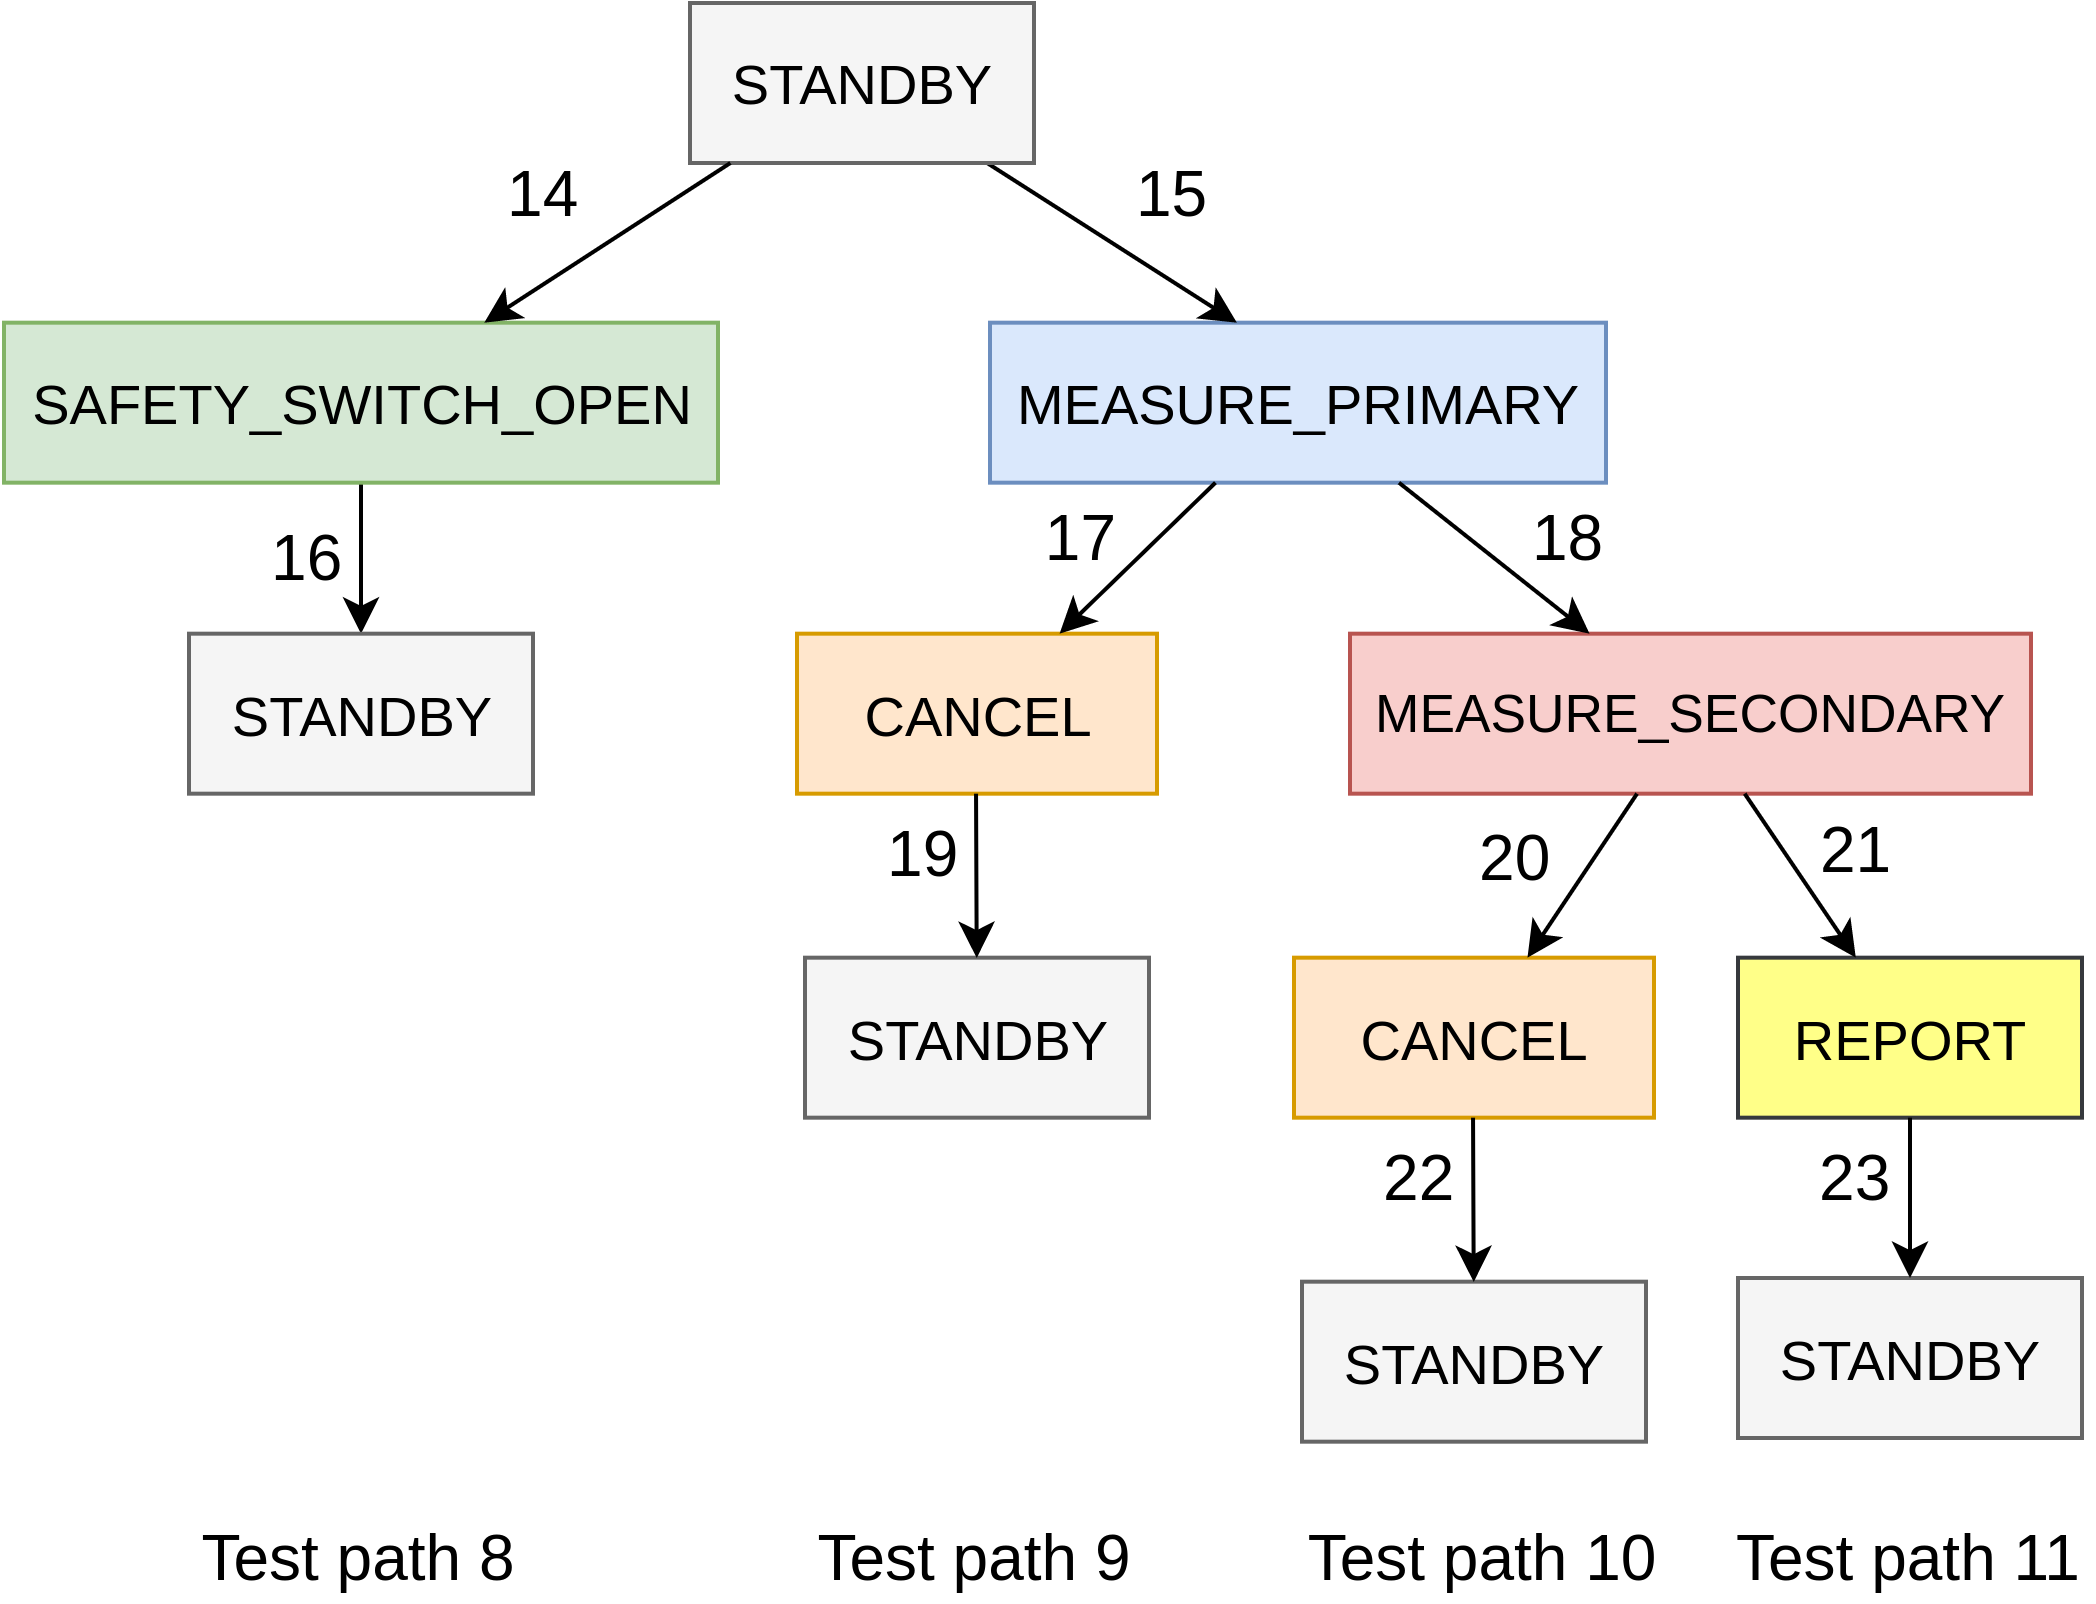
\includegraphics[scale=0.95]{./Figures/ArTrans_3.png}
	\caption{Árbol de transiciones: etapa de caracterización.}
	\label{fig:ArTrans_3}
\end{figure}

Para las pruebas de caracterización, se parte desde el estado STANDBY con el equipo configurado, por lo tanto, se tiene que superar el \textit{test path} 7 del estado de configuración para poder comenzar las pruebas de esta etapa.

A partir de estos ensayos, se pudieron validar los requerimientos: 
\begin{itemize}
\item Requerimientos 3 y 4 de la sección \ref{subsec:ReqFun}.
\item Requerimiento 3 de la sección \ref{subsec:ReqCom}.
\item Requerimientos 1.b, 1.c, 2.a, 2.b, 2.c, 2.d y 3 de la sección \ref{subsec:ReqUsu}.
\end{itemize}


\subsubsection{Prueba del \textit{test path} 8}
\label{subsubsec:pruCarac_8}

Condiciones iniciales: 

\begin{enumerate}
	\item Equipo energizado y \textit{test path} 7 corrido.
	\item Impresora encendida y conectada.
	\item Tapa de seguridad abierta.
\end{enumerate}

En la tabla \ref{tab:pruCarac_8}, se muestran los casos de pruebas para el \textit{test path} 8.

\begin{table}[htpb]
\centering
\caption[Prueba de la etapa de caracterización: \textit{test path} 8]{Casos de pruebas para el \textit{test path} 8.}
\resizebox{\textwidth}{!}{%
\begin{tabular}{cclc}
\hline
\toprule
\textbf{ID} & \textbf{Entrada}            & \textbf{Salida}  & \textbf{Estado}           \\
\midrule
-  & \begin{tabular}[c]{@{}c@{}}Tapa de seguridad\\ abierta \end{tabular}       & \begin{tabular}[c]{@{}l@{}}\textit{Display}: mostrar los datos del servidor web\\ \textit{Buzzer}: sin salida\\ Impresora: sin salida\end{tabular} & STANDBY           \\ \hline
14  & Pulsar Testear & \begin{tabular}[c]{@{}l@{}}\textit{Display}: ``Tapa de seguridad abierta''\\ \textit{Buzzer}: sin salida\\ Impresora: sin salida\end{tabular}      & SAFETY\_SWITCH\_OPEN \\ \hline
16  & -        & \begin{tabular}[c]{@{}l@{}}\textit{Display}: mostrar los datos del servidor web\\ \textit{Buzzer}: sin salida\\ Impresora: sin salida\end{tabular} & STANDBY          
\\ 
\bottomrule
\hline
\end{tabular}%
}
\label{tab:pruCarac_8}
\end{table}

Resultado: el ensayo se superó con éxito. En la figura \ref{fig:pruConf_8_res}, se muestran las imágenes obtenidas del \textit{display} para cada paso. 

\begin{figure}[!htpb]
     \centering
     \begin{subfigure}[b]{0.4\textwidth}
         \centering
         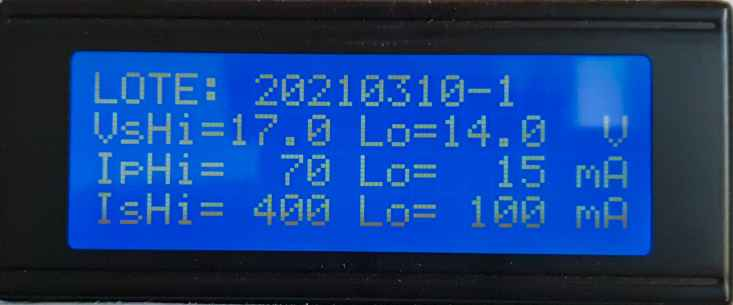
\includegraphics[width=1.1\textwidth]{./Figures/pru_fail.jpeg}
         \caption{STANDBY.}
         \label{fig:pruConf_8_1}
     \end{subfigure}
           \hfill
     \begin{subfigure}[b]{0.4\textwidth}
         \centering
         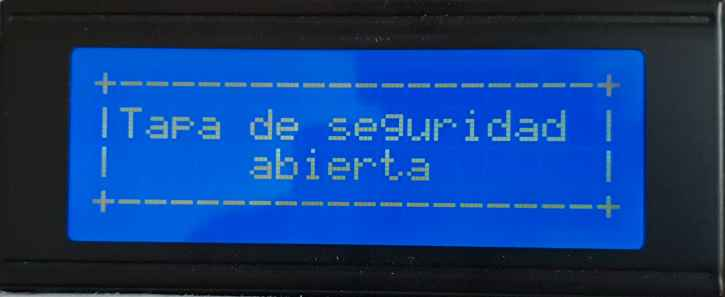
\includegraphics[width=1.1\textwidth]{./Figures/tapa_abierta.jpeg}
         \caption{SAFETY\_SWITCH\_OPEN.}
         \label{fig:pruConf_8_2}
     \end{subfigure}
           \hfill
     \begin{subfigure}[b]{0.4\textwidth}
         \centering
         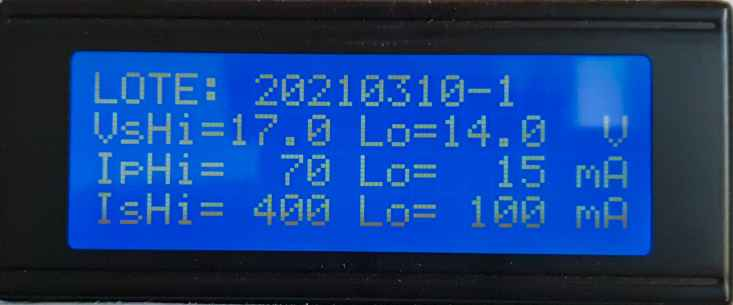
\includegraphics[width=1.1\textwidth]{./Figures/pru_fail.jpeg}
         \caption{STANDBY.}
         \label{fig:pruConf_8_3}
     \end{subfigure}
        \caption{Resultado del \textit{test path} 8.}
        \label{fig:pruConf_8_res}
\end{figure}

\subsubsection{Prueba del \textit{test path} 9}
\label{subsubsec:pruCarac_9}

Condiciones iniciales: 

\begin{enumerate}
	\item Equipo energizado y \textit{test path} 7 corrido.
	\item Impresora encendida y conectada.
	\item Tapa de seguridad cerrada.
\end{enumerate}

En la tabla \ref{tab:pruCarac_9}, se muestran los casos de pruebas para el \textit{test path} 9.

\begin{table}[htpb]
\centering
\caption[Prueba de la etapa de caracterización: \textit{test path} 9]{Casos de pruebas para el \textit{test path} 9.}
\resizebox{\textwidth}{!}{%
\begin{tabular}{cclc}
\hline
\toprule
\textbf{ID} & \textbf{Entrada}            & \textbf{Salida}  & \textbf{Estado}           \\
\midrule
-  & \begin{tabular}[c]{@{}c@{}}Tapa de seguridad\\ cerrada\end{tabular}      & \begin{tabular}[c]{@{}l@{}}\textit{Display}: mostrar los datos del servidor web\\ \textit{Buzzer}: sin salida\\ Impresora: sin salida\end{tabular} & STANDBY           \\ \hline
15 & Pulsar Testear                                                      & \begin{tabular}[c]{@{}l@{}}\textit{Display}: mostrar los datos del servidor web\\ \textit{Buzzer}: sin salida\\ Impresora: sin salida\end{tabular} & MEASURE\_PRIMARY \\ \hline
17 & Pulsar Cancelar                                                     & \begin{tabular}[c]{@{}l@{}}\textit{Display}: ``Cancelando espere...''\\ \textit{Buzzer}: sin salida\\ Impresora: sin salida\end{tabular}         & CANCEL           \\ \hline
19  & -        & \begin{tabular}[c]{@{}l@{}}\textit{Display}: mostrar los datos del servidor web\\ \textit{Buzzer}: sin salida\\ Impresora: sin salida\end{tabular} & STANDBY          
\\ 
\bottomrule
\hline
\end{tabular}%
}
\label{tab:pruCarac_9}
\end{table}

Resultado: el ensayo se superó con éxito. En la figura \ref{fig:pruConf_9_res}, se muestran las imágenes obtenidas del \textit{display} para cada paso. A partir de la misma secuencia de prueba, se probó la apertura de la tapa de seguridad una vez iniciado el ensayo, es decir, en vez de pulsar Cancelar en el paso 17, se procedió a abrir la tapa de seguridad y el resultado obtenido fue equivalente.

\begin{figure}[!htpb]
     \centering
     \begin{subfigure}[b]{0.4\textwidth}
         \centering
         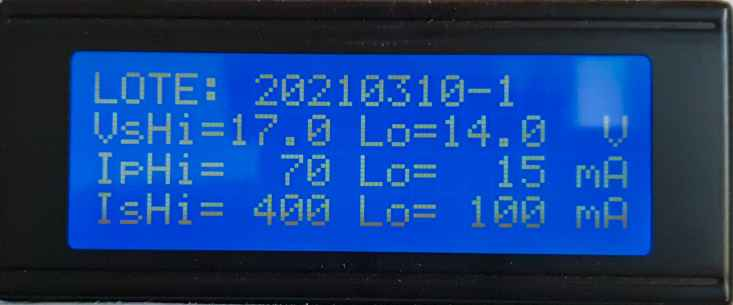
\includegraphics[width=1.1\textwidth]{./Figures/pru_fail.jpeg}
         \caption{STANDBY.}
         \label{fig:pruConf_9_1}
     \end{subfigure}
          \hfill
     \begin{subfigure}[b]{0.4\textwidth}
         \centering
         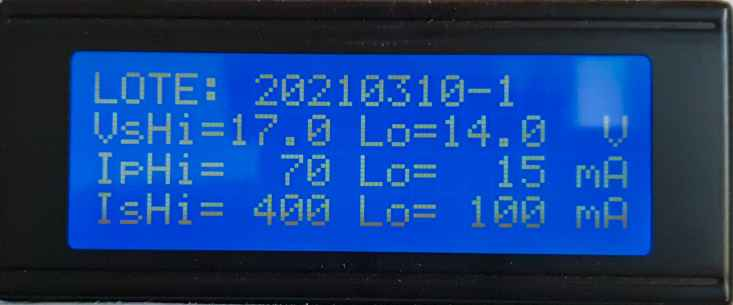
\includegraphics[width=1.1\textwidth]{./Figures/pru_fail.jpeg}
         \caption{MEASURE\_PRIMARY.}
         \label{fig:pruConf_9_2}
     \end{subfigure}
           \hfill
     \begin{subfigure}[b]{0.4\textwidth}
         \centering
         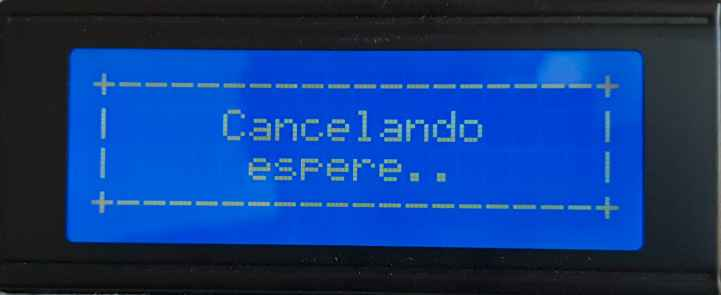
\includegraphics[width=1.1\textwidth]{./Figures/cancel.jpeg}
         \caption{CANCEL.}
         \label{fig:pruConf_9_3}
     \end{subfigure}
           \hfill
     \begin{subfigure}[b]{0.4\textwidth}
         \centering
         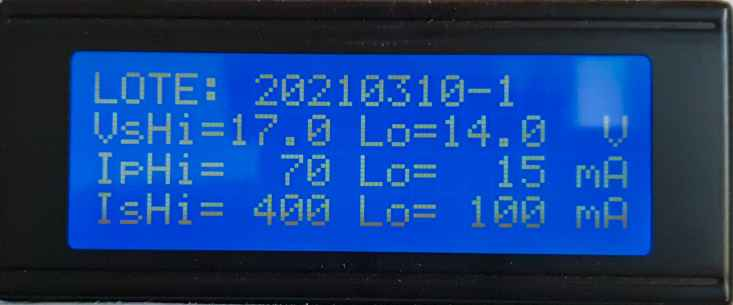
\includegraphics[width=1.1\textwidth]{./Figures/pru_fail.jpeg}
         \caption{STANDBY.}
         \label{fig:pruConf_9_4}
     \end{subfigure}
        \caption{Resultado del \textit{test path} 9.}
        \label{fig:pruConf_9_res}
\end{figure}

\subsubsection{Prueba del \textit{test path} 10}
\label{subsubsec:pruCarac_10}

Condiciones iniciales: 

\begin{enumerate}
	\item Equipo energizado y \textit{test path} 7 corrido.
	\item Impresora encendida y conectada.
	\item Tapa de seguridad cerrada.
\end{enumerate}

En la tabla \ref{tab:pruCarac_10}, se muestran los casos de pruebas para el \textit{test path} 10.

\begin{table}[htpb]
\centering
\caption[Prueba de la etapa de caracterización: \textit{test path} 10]{Casos de pruebas para el \textit{test path} 10.}
\resizebox{\textwidth}{!}{%
\begin{tabular}{cclc}
\hline
\toprule
\textbf{ID} & \textbf{Entrada}            & \textbf{Salida}  & \textbf{Estado}           \\
\midrule
-  & \begin{tabular}[c]{@{}c@{}}Tapa de seguridad\\ cerrada\end{tabular}      & \begin{tabular}[c]{@{}l@{}}\textit{Display}: mostrar los datos del servidor web\\ \textit{Buzzer}: sin salida\\ Impresora: sin salida\end{tabular} & STANDBY           \\ \hline
15 & Pulsar Testear                                                      & \begin{tabular}[c]{@{}l@{}}\textit{Display}: mostrar los datos del servidor web\\ \textit{Buzzer}: sin salida\\ Impresora: sin salida\end{tabular} & MEASURE\_PRIMARY \\ \hline
18 & -                                                      & \begin{tabular}[c]{@{}l@{}}\textit{Display}: mostrar los datos del servidor web\\ \textit{Buzzer}: sin salida\\ Impresora: sin salida\end{tabular} & MEASURE\_SECONDARY \\ \hline
20 & Pulsar Cancelar                                                     & \begin{tabular}[c]{@{}l@{}}\textit{Display}: ``Cancelando espere...''\\ \textit{Buzzer}: sin salida\\ Impresora: sin salida\end{tabular}         & CANCEL           \\ \hline
22  & -        & \begin{tabular}[c]{@{}l@{}}\textit{Display}: mostrar los datos del servidor web\\ \textit{Buzzer}: sin salida\\ Impresora: sin salida\end{tabular} & STANDBY          
\\ 
\bottomrule
\hline
\end{tabular}%
}
\label{tab:pruCarac_10}
\end{table}

Resultado: el ensayo se superó con éxito. Dado que los resultados son los mismos que en el ensayo anterior, se decidió omitir las figuras. Por otro lado, se probó la apertura de la tapa de seguridad siguiendo el mismo procedimiento que en el caso anterior.

\pagebreak

\subsubsection{Prueba del \textit{test path} 11}
\label{subsubsec:pruCarac_11}

Condiciones iniciales: 

\begin{enumerate}
	\item Equipo energizado y \textit{test path} 7 corrido.
	\item Impresora encendida y conectada.
	\item Servidor web en condiciones operativas.
	\item Tapa de seguridad cerrada.
\end{enumerate}

En la tabla \ref{tab:pruCarac_11}, se muestran los casos de pruebas para el \textit{test path} 11.

\begin{table}[htpb]
\centering
\caption[Prueba de la etapa de caracterización: \textit{test path} 11]{Casos de pruebas para el \textit{test path} 11.}
\resizebox{\textwidth}{!}{%
\begin{tabular}{cclc}
\hline
\toprule
\textbf{ID} & \textbf{Entrada}            & \textbf{Salida}  & \textbf{Estado}           \\
\midrule
-  & \begin{tabular}[c]{@{}c@{}}Tapa de seguridad\\ cerrada\end{tabular}      & \begin{tabular}[c]{@{}l@{}}\textit{Display}: mostrar los datos del servidor web\\ \textit{Buzzer}: sin salida\\ Impresora: sin salida\end{tabular} & STANDBY           \\ \hline
15 & Pulsar Testear                                                      & \begin{tabular}[c]{@{}l@{}}\textit{Display}: mostrar los datos del servidor web\\ \textit{Buzzer}: sin salida\\ Impresora: sin salida\end{tabular} & MEASURE\_PRIMARY \\ \hline
18 & -                                                      & \begin{tabular}[c]{@{}l@{}}\textit{Display}: mostrar los datos del servidor web\\ \textit{Buzzer}: sin salida\\ Impresora: sin salida\end{tabular} & MEASURE\_SECONDARY \\ \hline
21 & -                                                     & \begin{tabular}[c]{@{}l@{}}\textit{Display}: mostrar los resultados del ensayo\\ \textit{Buzzer}: emitir sonido acorde al \\ resultado del ensayo\\ Impresora: imprimir etiqueta acorde al \\ resultado del ensayo\end{tabular}         & REPORT           \\ \hline
23  & -        & \begin{tabular}[c]{@{}l@{}}\textit{Display}: mostrar los datos del servidor web\\ \textit{Buzzer}: sin salida\\ Impresora: sin salida\end{tabular} & STANDBY          
\\ 
\bottomrule
\hline
\end{tabular}%
}
\label{tab:pruCarac_11}
\end{table}

Dado que este ensayo es el encargado de probar que las mediciones y que las comparaciones se realicen apropiadamente, este se corrió varias veces con diferentes transformadores y diferentes datos en el servidor web. Con las variantes anteriores, se pudo verificar y validar que el equipo genere los resultados esperados para transformadores aprobados o rechazados.

En el primer caso, se realiza una prueba para un transformador rechazado. En la tabla \ref{tab:pruCarac_11_res}, se muestran los resultados esperados para este ensayo. En las columnas de máximo y mínimo se muestran los valores configurados desde el servidor web, los cuales, coinciden con los mostrados en la figura \ref{fig:serv_web_conf} del \textit{test path} 7.

\begin{table}[htpb]
\centering
\caption[Ensayo para transformador rechazado]{Resultados esperados para el \textit{test path} 11 en la condición de transformador rechazado}
\resizebox{0.6\textwidth}{!}{%
\begin{tabular}{ccccc}
\hline
\toprule
\textbf{Variable} & \textbf{Máximo} & \textbf{Mínimo} & \begin{tabular}[c]{@{}c@{}}\textbf{Valor}\\ \textbf{medido}\end{tabular} & \begin{tabular}[c]{@{}c@{}}\textbf{Resultado}\\ \textbf{esperado}\end{tabular} \\
\midrule
\begin{tabular}[c]{@{}c@{}}V$_{outS}$\\ {[}V{]}\end{tabular} & 17     & 14     & 17.7  & FALLA   \\
\begin{tabular}[c]{@{}c@{}}I$_{P}$\\ {[}mA{]}\end{tabular}   & 70     & 15     & 100   & FALLA   \\
\begin{tabular}[c]{@{}c@{}}I$_{S}$\\ {[}mA{]}\end{tabular}   & 400    & 100    & 977   & FALLA   \\                                                    
\bottomrule
\hline
\end{tabular}%
}
\label{tab:pruCarac_11_res}
\end{table}

Resultados para un transformador rechazado: el ensayo se superó con éxito. En la figura \ref{fig:pruConf_11_res_a}, se muestran las imágenes obtenidas del \textit{display} para cada paso.

\begin{figure}[!htpb]
     \centering
     \begin{subfigure}[b]{0.4\textwidth}
         \centering
         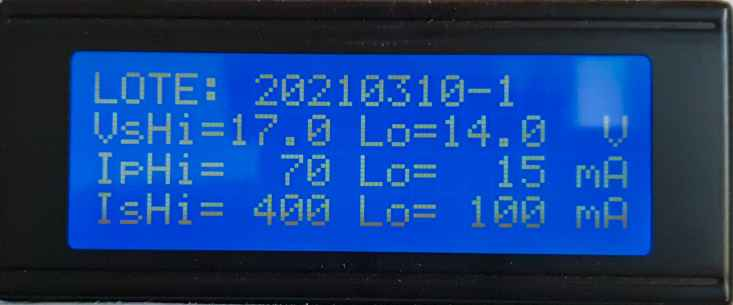
\includegraphics[width=1.1\textwidth]{./Figures/pru_fail.jpeg}
         \caption{MEASURE\_SECONDARY.}
         \label{fig:pruConf_11_1_a}
     \end{subfigure}
          \hfill
     \begin{subfigure}[b]{0.4\textwidth}
         \centering
         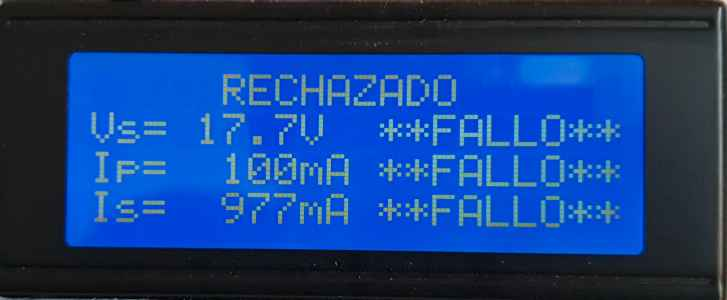
\includegraphics[width=1.1\textwidth]{./Figures/rechazado.jpeg}
         \caption{REPORT.}
         \label{fig:pruConf_11_2_a}
     \end{subfigure}
           \hfill
     \begin{subfigure}[b]{0.4\textwidth}
         \centering
         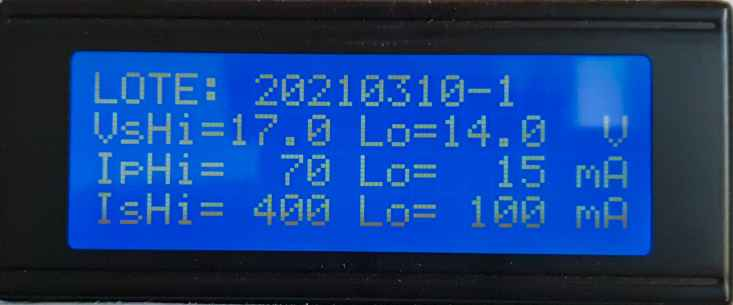
\includegraphics[width=1.1\textwidth]{./Figures/pru_fail.jpeg}
         \caption{STANDBY.}
         \label{fig:pruConf_11_3_a}
     \end{subfigure}
        \caption{Resultado del \textit{test path} 11 en el caso de un transformador rechazado.}
        \label{fig:pruConf_11_res_a}
\end{figure}

En el paso 21, ya se dispone de los valores medidos y del resultado de la caracterización. En este paso, se verificó que estos valores, mostrados en el \textit{display} en la figura \ref{fig:pruConf_11_2_a}, sean iguales a los enviados al servidor web que se muestran en la figura \ref{fig:serv_web_falla_resul} e iguales a los impresos en la etiqueta que se observan en la figura \ref{fig:etiqueta_falla}. Finalmente, todos estos valores coinciden con los presentados en la tabla \ref{tab:pruCarac_11_res} al inicio de la prueba.

\begin{figure}[htpb]
	\centering
	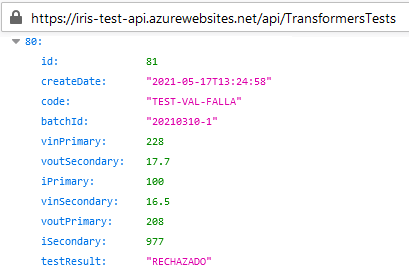
\includegraphics[scale=0.9]{./Figures/serv_web_falla_resul.png}
	\caption{Valores recibidos en el servidor web para el \textit{test path} 11 en el caso de un transformador rechazado.}
	\label{fig:serv_web_falla_resul}
\end{figure}

\begin{figure}[htpb]
	\centering
	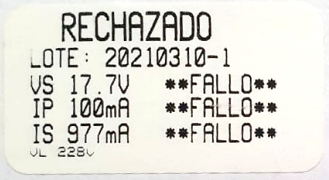
\includegraphics[scale=0.7]{./Figures/etiqueta_falla.png}
	\caption{Etiqueta resultante del \textit{Test path} 11 en el caso de un transformador rechazado.}
	\label{fig:etiqueta_falla}
\end{figure}

\pagebreak

A continuación, se procede a realizar una prueba para un transformador aprobado. Para realizar este ensayo, primero se debe configurar el equipo con nuevos valores de comparación, de forma tal, que los valores medidos estén dentro de los valores a comparar y permitan que el ensayo sea aprobado. Para reconfigurar el equipo, se deben guardar los valores indicados en la figura \ref{fig:serv_web_ok_conf} en el servidor web y luego se debe llevar a cabo el \textit{test path} 7 nuevamente.

\begin{figure}[htpb]
	\centering
	\includegraphics[scale=0.9]{./Figures/serv_web_ok_conf.png}
	\caption{Nuevos datos de configuración en el servidor web.}
	\label{fig:serv_web_ok_conf}
\end{figure}

En la tabla \ref{tab:pruCarac_11_res_apro}, se muestran los resultados esperados para este ensayo en función de los nuevos umbrales de comparación.

\begin{table}[htpb]
\centering
\caption[Ensayo para transformador aprobado]{Resultados esperados para el \textit{test path} 11 en la condición de transformador aprobado}
\resizebox{0.6\textwidth}{!}{%
\begin{tabular}{ccccc}
\hline
\toprule
\textbf{Variable} & \textbf{Máximo} & \textbf{Mínimo} & \begin{tabular}[c]{@{}c@{}}\textbf{Valor}\\ \textbf{medido}\end{tabular} & \begin{tabular}[c]{@{}c@{}}\textbf{Resultado}\\ \textbf{esperado}\end{tabular} \\
\midrule
\begin{tabular}[c]{@{}c@{}}V$_{outS}$\\ {[}V{]}\end{tabular} & 18     & 16     & 17.6  & OK   \\
\begin{tabular}[c]{@{}c@{}}I$_{P}$\\ {[}mA{]}\end{tabular}   & 110    & 90     & 100   & OK   \\
\begin{tabular}[c]{@{}c@{}}I$_{S}$\\ {[}mA{]}\end{tabular}   & 1100   & 900    & 969   & OK   \\                                                    
\bottomrule
\hline
\end{tabular}%
}
\label{tab:pruCarac_11_res_apro}
\end{table}

\pagebreak

Resultados para un transformador aprobado: el ensayo se superó con éxito. En la figura \ref{fig:pruConf_11_res_b}, se muestran las imágenes obtenidas del \textit{display} para cada paso, en la figura \ref{fig:serv_web_ok_resul} se muestran los datos enviados al servidor web y en la figura \ref{fig:etiqueta_OK} se muestra la etiqueta impresa.

\begin{figure}[!htpb]
     \centering
     \begin{subfigure}[b]{0.4\textwidth}
         \centering
         \includegraphics[width=1.1\textwidth]{./Figures/pru_pass.jpeg}
         \caption{STANDBY - MEASURE.}
         \label{fig:pruConf_11_1_b}
     \end{subfigure}
          \hfill
     \begin{subfigure}[b]{0.4\textwidth}
         \centering
         \includegraphics[width=1.1\textwidth]{./Figures/aprobado.jpeg}
         \caption{REPORT.}
         \label{fig:pruConf_11_2_b}
     \end{subfigure}
           \hfill
     \begin{subfigure}[b]{0.4\textwidth}
         \centering
         \includegraphics[width=1.1\textwidth]{./Figures/pru_pass.jpeg}
         \caption{STANDBY.}
         \label{fig:pruConf_11_3_b}
     \end{subfigure}
        \caption{Resultado del \textit{test path} 11 en el caso de un transformador aprobado.}
        \label{fig:pruConf_11_res_b}
\end{figure}

Al igual que en el ensayo para el transformador rechazado, en este caso, todos los valores obtenidos coinciden con los presentados en la tabla \ref{tab:pruCarac_11_res_apro}.

\pagebreak

\begin{figure}[htpb]
	\centering
	\includegraphics[scale=0.9]{./Figures/serv_web_ok_resul.png}
	\caption{Valores recibidos en el servidor web para el \textit{test path} 11 en el caso de un transformador aprobado.}
	\label{fig:serv_web_ok_resul}
\end{figure}

\begin{figure}[htpb]
	\centering
	\includegraphics[scale=0.7]{./Figures/etiqueta_OK.png}
	\caption{Etiqueta resultante del \textit{test path} 11 en el caso de un transformador aprobado.}
	\label{fig:etiqueta_OK}
\end{figure}


\subsection{Pruebas de la etapa de reporte}

Finalmente, se probó la etapa de reporte. Para esta etapa, se armó el árbol de transiciones mostrado en la figura \ref{fig:ArTrans_4}. A partir de este, se obtuvieron cuatro caminos a verificar: \textit{test path} 12 a 14. Para este caso, se muestra solo la tabla \ref{tab:pruRepor_12} que corresponde al camino 12, ya que, las demás tablas son idénticas a esta y solo cambia el mensaje de error.

\begin{figure}[htpb]
	\centering
	\includegraphics[scale=1]{./Figures/ArTrans_4.png}
	\caption{Árbol de transiciones: etapa de reporte.}
	\label{fig:ArTrans_4}
\end{figure}

Para las pruebas de reporte se parte desde el estado REPORT. Para arribar a este estado, se debe correr el \textit{test path} 11 de las pruebas de la etapa de caracterización.

A partir de estos ensayos, se pudieron validar los requerimientos: 
\begin{itemize}
\item Requerimiento 4 de la sección \ref{subsec:ReqFun}.
\item Requerimiento 3 de la sección \ref{subsec:ReqCom}.
\item Requerimiento 2.d de la sección \ref{subsec:ReqUsu}.
\end{itemize}

\pagebreak

\subsubsection{Prueba del \textit{test path} 12}
\label{subsubsec:pruRepor_12}

Condiciones iniciales: 

\begin{enumerate}
	\item Equipo energizado y \textit{test path} 11 corrido.
	\item Impresora desenergizada.
\end{enumerate}

En la tabla \ref{tab:pruRepor_12}, se muestran los casos de pruebas para el \textit{test path} 12.

\begin{table}[htpb]
\centering
\caption[Prueba de la etapa de reporte: \textit{test path} 12]{Casos de pruebas para el \textit{test path} 12.}
\resizebox{\textwidth}{!}{%
\begin{tabular}{cclc}
\hline
\toprule
\textbf{ID} & \textbf{Entrada}            & \textbf{Salida}  & \textbf{Estado}           \\
\midrule
-  & \begin{tabular}[c]{@{}c@{}}Impresora apagada\end{tabular}      & \begin{tabular}[c]{@{}l@{}}\textit{Display}: mostrar los datos del servidor web\\ \textit{Buzzer}: sin salida\\ Impresora: -\end{tabular} & STANDBY           \\ \hline
15 & Pulsar Testear                                                      & \begin{tabular}[c]{@{}l@{}}\textit{Display}: mostrar los datos del servidor web\\ \textit{Buzzer}: sin salida\\ Impresora: -\end{tabular} & MEASURE\_PRIMARY \\ \hline
18 & -                                                      & \begin{tabular}[c]{@{}l@{}}\textit{Display}: mostrar los datos del servidor web\\ \textit{Buzzer}: sin salida\\ Impresora: -\end{tabular} & MEASURE\_SECONDARY \\ \hline
21 & -                                                     & \begin{tabular}[c]{@{}l@{}}\textit{Display}: mostrar los resultados del ensayo\\ \textit{Buzzer}: emitir sonido acorde al \\ resultado del ensayo\\ Impresora: -\end{tabular}         & REPORT           \\ \hline
24 & -                                                      & \begin{tabular}[c]{@{}l@{}}\textit{Display}: ``Fallo de COM con impresora''\\ \textit{Buzzer}: emitir sonido acorde al \\ resultado del ensayo\\ Impresora: -\end{tabular} & \begin{tabular}[c]{@{}c@{}}REPORT\\(printer failure)\end{tabular}  \\ \hline
27  & -        & \begin{tabular}[c]{@{}l@{}}\textit{Display}: mostrar los datos del servidor web\\ \textit{Buzzer}: sin salida\\ Impresora: -\end{tabular} & STANDBY          
\\ 
\bottomrule
\hline
\end{tabular}%
}
\label{tab:pruRepor_12}
\end{table}

Resultado: el ensayo se superó con éxito. En la figura \ref{fig:pruConf_12_res}, se muestran las imágenes obtenidas del \textit{display} para cada paso, se omiten las capturas de los primeros cuatro pasos ya que son iguales a los del \textit{test path} 11.

\begin{figure}[!htpb]
     \centering
     \begin{subfigure}[b]{0.4\textwidth}
         \centering
         \includegraphics[width=1.1\textwidth]{./Figures/falla_com_printer.jpeg}
         \caption{REPORT (printer failure).}
         \label{fig:pruConf_12_1}
     \end{subfigure}
          \hfill
     \begin{subfigure}[b]{0.4\textwidth}
         \centering
         \includegraphics[width=1.1\textwidth]{./Figures/pru_pass.jpeg}
         \caption{STANDBY.}
         \label{fig:pruConf_12_2}
     \end{subfigure}
        \caption{Resultado del \textit{test path} 12.}
        \label{fig:pruConf_12_res}
\end{figure}

\subsubsection{Prueba de los \textit{test paths} 13 y 14}
\label{subsubsec:pruRepor_13}

Para el camino 13 las condiciones iniciales son las siguientes:
\begin{enumerate}
	\item Equipo energizado y \textit{test path} 11 corrido.
	\item Impresora encendida y conectada.
	\item \textit{Router} Wi-Fi apagado.
\end{enumerate}

En el \textit{display} se debe leer ``Fallo al enviar reporte al webserv'' para luego mostrar ``Falla Web Server Equipo bloqueado''. En al figura \ref{fig:pruConf_13_res}, se muestran las imágenes obtenidas para este caso.

\begin{figure}[!htpb]
     \centering
     \begin{subfigure}[b]{0.4\textwidth}
         \centering
         \includegraphics[width=1.1\textwidth]{./Figures/falla_web_server.jpeg}
         \caption{REPORT (web server failure).}
         \label{fig:pruConf_13_1}
     \end{subfigure}
          \hfill
     \begin{subfigure}[b]{0.4\textwidth}
         \centering
         \includegraphics[width=1.1\textwidth]{./Figures/Sin_Conex_WiFi_Eq_Bloq.jpeg}
         \caption{BLOCK\_DEVICE.}
         \label{fig:pruConf_13_2}
     \end{subfigure}
        \caption{Resultado del \textit{test path} 13 y 14.}
        \label{fig:pruConf_13_res}
\end{figure}

Por otro lado, para el camino 14 las condiciones iniciales son las siguientes:
\begin{enumerate}
	\item Equipo energizado y \textit{test path} 11 corrido.
	\item Impresora encendida y conectada.
	\item \textit{Router} Wi-Fi funcionando.
	\item Servidor web no disponible.
\end{enumerate}

Finalmente, en el \textit{display} se leen los mismos mensajes que en el caso anterior.